\documentclass{article}
\setlength{\headheight}{13.59999pt}
\usepackage[utf8]{inputenc}

\title{Luminosity function}
\author{Henrik Andrews}

\usepackage{natbib}

\usepackage{subcaption}
\usepackage[ portrait, margin=2cm]{geometry}
\usepackage{graphicx}
\usepackage{amsmath}
\usepackage{upgreek}
\usepackage{bbold}
\usepackage{fancyhdr}
\usepackage{mathtools}
\usepackage{tabularx}
\usepackage{lipsum}
\usepackage{pdfpages}
\setlength{\parindent}{0em}
\setlength{\parskip}{1em}
\usepackage{caption}
\usepackage{multicol}

\usepackage{float}
\newcommand{\HRule}[1]{\rule{\linewidth}{#1}}
\usepackage{listings}
\usepackage{color} %red, green, blue, yellow, cyan, magenta, black, white
\definecolor{mygreen}{RGB}{28,172,0} % color values Red, Green, Blue
\definecolor{mylilas}{RGB}{170,55,241}
\definecolor{backcolour}{rgb}{0.95,0.95,0.92}
\begin{document}

% title source: https://www.overleaf.com/project/6021d9e4632b9ef90aa8d238
\title{ \normalsize \textsc{AREA}
	\\ [2.0cm]
	\HRule{0.5pt} \\
	\LARGE \textbf{\uppercase{Theme}}		
	\\ Title\\
	\HRule{2pt} \\ [0.5cm]		
%fix the university logo !!!!!!!!!!!!!!!!!!!!!!!!
	\vspace{6cm}
	\begin{figure}[htp]
    \centering
    
\includegraphics[width=.2\textwidth]{Logo-Ntnu.svg.png}
    \end{figure}
	}

\author{
    \normalsize 
	\textbf{Henrik Døvle Andrews } \\
	Norwegian university of Science and Technology \\ 
}

\maketitle
\setcounter{page}{ 0 }

\newpage

\pagestyle{fancy}
\fancyhf{}
\setlength\headheight{12pt}
\fancyhead[L]{Henrik Døvle Andrews}
\fancyhead[R]{Luminosity functions}
\fancyfoot[R]{Page \thepage \:}
\setcounter{page}{1}


\maketitle

% Abstract
\begin{abstract}
\lipsum[1] % Replace with your abstract text
\end{abstract}

\newpage 
% Summary (you might use a simple section for this)
\section*{Summary}
\lipsum[2] % Replace with your summary text

\newpage
% Acknowledgments
\section*{Acknowledgments}
\lipsum[3] % Replace with your acknowledgment text

\newpage
% Table of Contents (optional)
\tableofcontents

\newpage
% List of Figures
\listoffigures

% List of Tables
\listoftables

-abstract 
-sammendrag
-acknowledgments
-list of figure
-list of tables

\newpage


\section{Introduction}


\section{The ever-expanding Universe}
To investigate sources very far away from an observer it is important to understand the influence this distance 
has on the desired observables. Therefore in astrophysics and astronomy in general there are distances created to take into account the effects of an expanding Universe. 


\subsection{Cosmological parameters}

A reasonable place to start is with the Hubble constant $H_0$. 
This parameter sets the recession speed of a point at proper distance $d$ and the current position via this relation. $v = H_0 d$ 
The subscript $0$ refers to the present epoch signifying that $H_0$ is not static but changes with time. 
The precise value of $H_0$ is quite debated so it's commonly expressed in a parameterised form,
$$
H_0= 100\frac{\rm km}{\rm s}\frac{1}{\rm Mpc} h.
$$
The parameter $h$ is a dimensionless number that according to current knowledge can take the value between $0.5$ to $0.8$ reflecting the range of answers collected from recent work. 

Beyond its basic definition,$H_0$ also allows for the derivation of two significant cosmic scales:

\textbf{Hubble Time ($t_H$) }: Defined as the inverse of 
$H_0$, $t_H$ provides an estimate of the age of the Universe. 
It sets a scale for the time since the Big Bang, assuming the Universe has been expanding at a constant rate. The equation 
$t_H = \frac{1}{H_0} \approx 14 \quad \text{Billion years}$ offers a way to approximate this expansive timescale.


\textbf{Hubble Distance ($D_H$) }: This is a measure of the distance over which the Universe's expansion is significant. Calculated as 
$D_H = \frac{c}{H_0} \approx 4.4 \quad \text{Gly}$, where $c$ is the speed of light, 
it represents a critical boundary in observational cosmology. %Beyond this distance, the expansion of the Universe dominates the motion of galaxies, providing a fundamental constraint for cosmological observations and theories.

\subsection{Shape of the Universe}


The shape and expansion of the Universe are central themes in cosmology, but first one needs to define the structure of the Universe and its contents. 
In this paper and many articles, the Universe is
often explored through the lens of the flat Lambda Cold Dark Matter ($\Lambda$CDM) model. 
This model, widely accepted in contemporary cosmology, provides a framework for understanding the Universe's composition and its expansion dynamics by assuming as the name suggests no curvature.
In the $\Lambda$CDM model, two key parameters are important: the mass density of the Universe, $\rho_0$, and the cosmological constant, $\Lambda$.
These parameters, which evolve, are a part of defining the metric tensor in general relativity, thereby allowing us to model the curvature of the Universe based on its initial conditions.
These parameters are often expressed as dimensionless variables:

$$
\Omega_m = \frac{8\pi G\rho_0}{3H_0^2}
$$

$$
\Omega_\Lambda = \frac{\Lambda c^2}{3H_0^2}
$$

Here, $\Omega_m$ represents the matter density parameter, encompassing both ordinary (baryonic) matter and dark matter. 
$\Omega_\Lambda$, on the other hand, corresponds to the density parameter associated with the cosmological constant, which is often interpreted as dark energy.




In general, one has a third density parameter $\Omega_k$ which defines the curvature of space time and the relationship between these parameters is expressed as: 

$$
\Omega_m + \Omega_\Lambda + \Omega_k = 1
$$


In a flat Universe, one has $\Omega_k = 0$ and the Universe is dominated by dark energy and dark matter. The model used in this paper and the papers cited if not expressed otherwise is the flat $\Lambda$CDM model where the parameters take the values of 
$\Omega_\Lambda = 0.7$ and $\Omega_m = 0.3$. These values align with current observational data.



\subsection{Redshift}
Redshift is defined as the fractional Doppler shift of emitting light. The Doppler effect is a known effect on different observables in the Universe where the relative motion of sources to observers will impact the observable. The redshift is quantified for a light source as 

\begin{equation}
    z = \frac{\nu_e}{\nu_o}-1 = \frac{\lambda_o}{\lambda_e}-1
\end{equation}

Here $o$ refers to the observed quantity and $e$ the emitted. Due to the expansion of the Universe the light emitted from a distant source will be increasingly redshifted the further away it is.
In these scenarios the redshift serves as a distance measure, allowing us to deduce distances to faraway objects.



\subsection{Comoving distance}
\label{sec:comoving_distance}


Comoving distance is an important concept in cosmography, 
acting as a standard unit for various distance measurements in the Universe. 
This distance, often termed the line-of-sight distance for an observer on Earth, 
remains constant even as objects expand with the Hubble flow. 
To calculate the total comoving distance ($D_c$) to an object, 
one integrates the differential comoving distances ($\delta D_c$) along the line of sight, starting from redshift 
$z=0$ to the object. This integration necessitates consideration of the Universe's parametric composition and the $\delta D_c$ is expressed as

\begin{equation}
    \delta D_c = \frac{D_H}{E(z)}dz
\end{equation}
where the function $E(z)$ is defined as
\begin{equation}
    E(z)  = \sqrt{\Omega_m(z+1)^3 +\Omega_k (1+z)^2 + \Omega_\Lambda  }
\end{equation}
Here, 
$E(z)$ incorporates the density parameters previously discussed and the redshift 
$z$. It also relates to the Hubble constant observed by a hypothetical observer at redshift $z$, expressed as 
$H(z) = H_0 E(z)$.

One then receives the comoving distance $D_c$ from 
\begin{equation}
    D_c =D_H \int_0^z\frac{dz}{E(z)}
\end{equation}

In addition to the line of sight, one needs to define the transverse comoving distance $D_m$. This distance 
relates two points in the night sky at the same redshift separated by an angle $d\theta$. The actual distance
between them $d\theta D_m$ will then vary depending on the curvature of the Universe. This relationship is summarised in the following equation
which accounts for different geometries,

$$
D_m =
\begin{cases}
  D_h\frac{1}{\sqrt{\Omega_k}}sinh(\frac{\sqrt{\Omega_k}D_c}{D_H}) & \text{if } \Omega_k > 0 \\
  D_c& \text{if } \Omega_k = 0 \\
  D_h\frac{1}{\sqrt{|\Omega_k|}}sin(\frac{\sqrt{|\Omega_k|}D_c}{D_H}) & \text{if } \Omega_k < 0
\end{cases}
$$

The different cases correspond to hyperbolic, flat, and spherical geometry respectively. The true nature 
of the Universe is still unknown but the recent observations indicate a flat universe. 








\subsection{Luminosity distance}
The luminosity distance $D_l$ is defined through the relation between 
the bolometric flux $F$ of a source and its bolometric luminosity $L$. bolometric flux is the energy received per unit of time per unit area, while bolometric luminosity is the total energy emitted per unit of time.
The luminosity distance is defined as
\begin{equation}
    D_l = \sqrt{\frac{L}{4\pi F}}
\end{equation}

This formula essentially describes the loss of energy due to the expansion of the Universe. It reflects how the observed flux at the observer's location differs based on the distance from the source and the intrinsic luminosity emitted. 

It is related to the transverse comoving distance via 

\begin{equation}
    D_l = (1+z)D_m
\end{equation}

This of course is for bolometric quantities, but if one wants to calculate the spectral 
flux/ differential flux one needs to take into account a correction. This correction comes 
from the fact that one is viewing a redshifted object. The object is emitting in a different band than 
observed. The spectrum of the differential flux $F_\nu$ is related to the spectral luminosity via
\begin{equation}
    F_\nu = (1+z) \frac{L_{(1+z)\nu}}{L_\nu}\frac{L_\nu}{4\pi D_l^2}
\end{equation}


All these equations listed help include the effects of an expanding universe when astronomers study distant objects and their properties. 

\section{High energy particles}
In this section, I will discuss the different types of high-energy particles that are of interest in this paper, i.e. neutrinos and ultra-high energy cosmic rays(UHECRs).
I will briefly discuss their generation and how they are detected. Then introduce how they lose energy in their journey to earth, and lastly calculate the emissivity of their hypothetical sources from the ground 
observations here on earth. 

\subsection{Acceleration of high energy particles}

To reach high energy, particles need to be accelerated. 
Knowing the exact source of acceleration can be difficult since we do not know the sources, but one can put constraints on any source given some simple arguments.
By arguing that the acceleration needs to be of a certain strength and that the particle being accelerated needs to stay confined within the accelerator for long enough one can put constraints on the source.
This is called the Hillas criterion and is a way of estimating the maximum energy a particle can reach in a given source.% (ref hillas)

For relativistic particles with charge $Z$ and energy $\epsilon$ in a magnetic field of strength $B$ one can define the Larmor radius


\begin{equation}
    R_L = \frac{\epsilon}{ZB}
\end{equation}

By arguing that the definition of confinement of a particle to a source is by equating the Larmor radius to the size of the source one can 
easily derive the maximum achievable energy for a particle as follows.% (ref M. Bustamante. https://cds.cern.ch/record/1249755/files/p533.pdf)

\begin{equation}
    \epsilon_{max} = ZBR
\end{equation}

Via this method, one can illustrate the potential candidates needed to produce the required and importantly observed high-energy particles. 
This requirement is named the Hillas criterion after G. Hillas who first proposed this method.
In figure \ref{fig:hillas_c} one can see the different candidates for the acceleration of two different ions, protons, and iron. One of the candidates is the AGN, which is the focus of this paper.

\begin{figure}
    \centering
    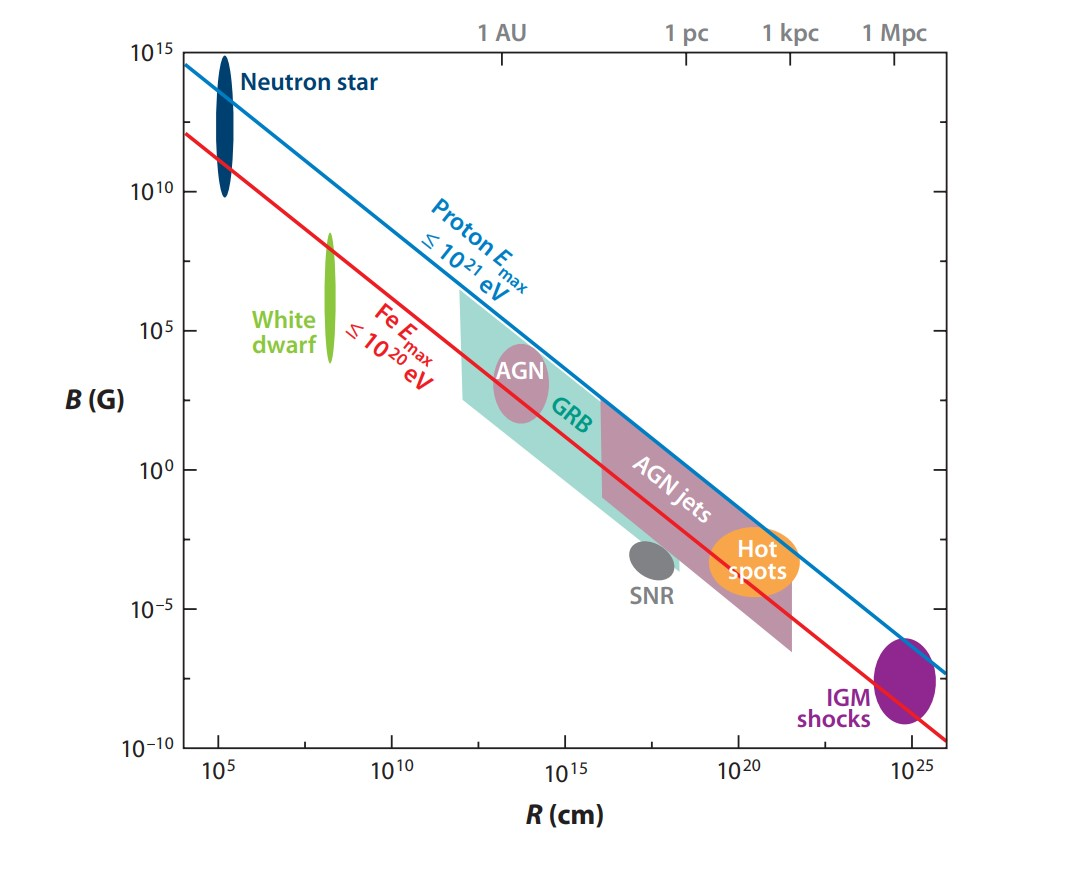
\includegraphics[width = 0.5\textwidth]{hillas_criterion.jpeg}
    \caption{Hillas criterion for proton (blue line) and iron (red line) accelerated up to $10^{20}eV$ and $10^{21}eV$ respectively. Image taken from \cite{doi:10.1146/annurev-astro-081710-102620}}
    \label{fig:hillas_c}
\end{figure}


One can try to build sources in bottom-up models, and then it is necessary to understand the different processes that can accelerate particles to high energies, here I will briefly go through some. 

\textbf{One-shot acceleration}:
In the presence of an ordered field, one can continuously accelerate particles. This could be the feature of some astrophysical objects such as neutron stars and black holes.% (ref cern paper)


\textbf{Diffusive acceleration/ Fermi acceleration}
In regions where one has high variability in the magnetic field strength, one can accelerate particles in burst. 
This is called diffusive acceleration and the most common way of this happening is through first and second-order Fermi acceleration.
The second-order Fermi acceleration is the simplest and is based on the fact that particles can gain energy by bouncing back and forth between magnetic clouds which act as mirrors. 
This is a stochastic process and the average energy gain can be shown to be proportional $(\frac{v}{c})^2$. Here $v$ is the speed of the cloud 
and $c$ is the speed of the particle. This is a slow process due to the scarcity of clouds and therefore it is not a preferred method.
The first-order Fermi acceleration happens when particles collide with strong shock fronts. These shock fronts can be quite a bit faster than the interstellar clouds
and when a particle moves through the shock it gains energy proportional to $\frac{v}{c}$. In addition to this, there is a probability that the particle will stay in the accelerating region and 
experience several shocks accelerations. 

By knowing how particles can accelerate and their potential sources one can continue an look at the two particles in question in this paper. 
Neutrinos and UHECRs.
\subsection{UHECRs}

UHECRs are simply put charged particles that are bombarding the Earth with energy exceeding .... (1exaelectronvolt ($10^{18}$ eV)). The origin of 
these particles are still a mystery but due to their high energies, they are thought to be extragalactic in origin and due to the Hillas criterion need to be sufficiently good accelerators.
The composition of UHECRs is mostly protons and heavier nuclei such as helium or iron, and when these particles interact with the atmosphere they produce a shower of secondary particles.
The air showers could also give extra information such as direction, but due to the nature of UHECRs, the location of their source is
difficult to pinpoint. This is because UHECRs are charged particles and therefore are deflected by the magnetic fields they encounter.

\subsubsection{Production and Energy loss}
The requirements to produce a UHECR are a charged particle and a powerful accelerator. From the Hillas criterion, one can see that there are several candidates so I will assume that these requirements are fulfilled and we have a particle with sufficient energy that has been released from its source.
An equally interesting part is the journey of the particle to Earth since during the acceleration and during the journey to Earth, the UHECRs will lose energy. The important parameters for this energy loss are its composition and its environment. In addition, as mentioned before, the interstellar magnetic field will also deflect the particles and therefore the direction of the particle will be changed. These effects are important parameters since they limit the 
distance a particle can travel before its start energy becomes unreasonable, and therefore limits the local volume in which it can be produced. 
Here I will briefly discuss the different energy loss mechanisms. 
\textbf{Photo-pair production}

\begin{equation}
    p + \gamma \rightarrow p + e^- + e^+
\end{equation}
For UHECRs, the most potent sink of energy is the Bethe-Heitler process. In this process, a proton of sufficient energy interacts with the 
photon field in its vicinity and produces a pair of electrons and positrons. The photon field can vary from the cosmic microwave background to the generated field from different sources. 
The energy loss of this process is quite small $\sim \frac{2m_e}{m_p}= 10^{-3}$ of the original energy of the proton, but the process is very common and therefore it is a significant energy loss over time.


\textbf{Pion production through delta resonance}
\begin{equation}
    p + \gamma \rightarrow \Delta^+ \rightarrow (p + \pi^0)\quad \text{or} \quad (\pi^+ + n)
    \label{eq:delta_resonance}
\end{equation}

Given enough energy the proton can interact with the photon field and produce a delta resonance. This resonance can then decay into a pion and a proton or a neutron and a pion. 
This process is important since it also puts an upper limit on the UHECR energy for intergalactic particles. 
This limit, called the Greisen-Zatsepin-Kuzmin (GZK) limit comes from the UHECRs interacting with the cosmic microwave background in this delta resonance process. The limit caps proton energy at $5\times 10^{19}$ eV.

%\textbf{photodisintegration}
%mabye include this. 

\subsubsection{Detection}
When a cosmic ray hits the atmosphere it will interact with the air molecules and produce a cascade of particles and light that can more easily be detected than 
the original cosmic ray. In addition, since the UHECR flux at high energy is extremely low (<1 particle per $km^2$ per year for $E > 10^{19}$ ) one needs a large area to collect enough data. 
The best detectors to do this kind of work are the Pierre Auger Observatory and the Telescope Array. 

The Pierre Auger Observatory is located in Argentina and is the largest detector of its kind. It consists of 1660  Cherenkov detectors spread over 3000 km$^2$ and 27 fluorescence telescopes in four locations. With 
these instruments, the observatory is very capable of reconstructing the air showers and therefore the original cosmic ray. The observatory has a blind spot in the night sky 
and therefore the observatory is complemented by the Telescope Array located in Utah. The Telescope Array is a smaller observatory with 507 scintillator detectors and 3 fluorescence telescopes. Combined they have been able to map the full sky of UHECRs.  

\subsubsection{Emissivity estimates}
\label{sec:emmisivity}

Now that one reasonably understands the nature of UHECRs one can try to make tangible estimates of the UHECRs sources. One such
estimate is the emissivity of UHECR sources. An emissivity is a measure of the energy released per unit time per unit volume. The question 
one can ask ourselves is what is the neceassary emissivity of UHECRs to explain the observed flux here on Earth? In other words, what is the required energy injection rate of IHECRs?


\begin{figure}
    \centering
    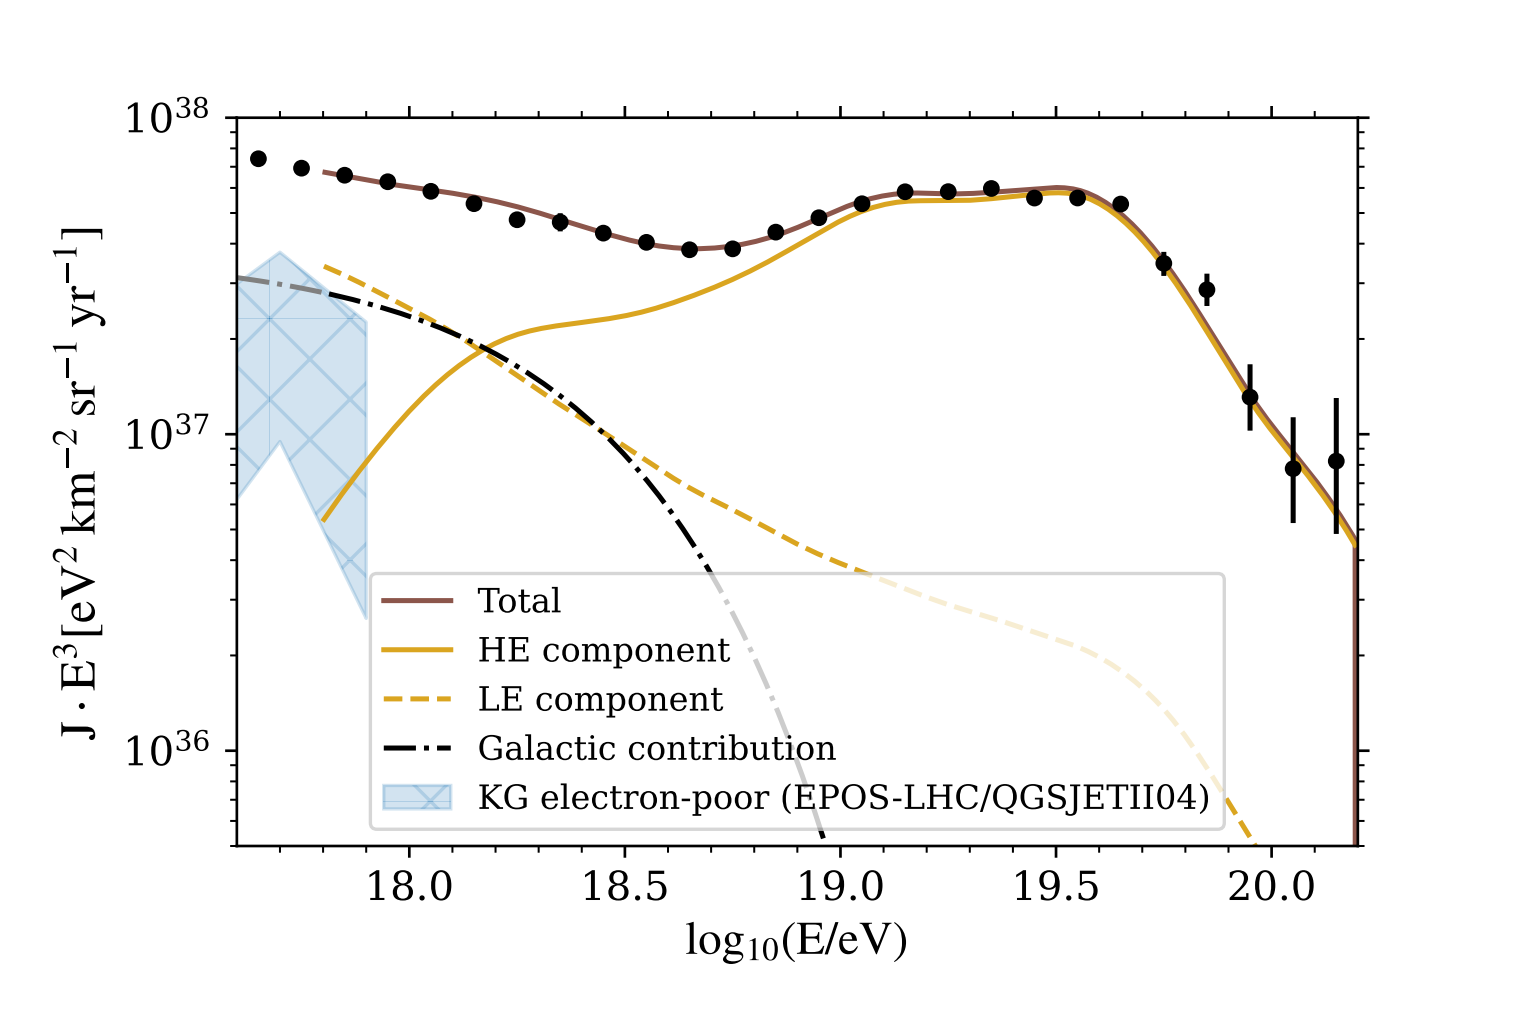
\includegraphics[width = 0.7\textwidth]{UHECRs.png}
    \caption{The diffuse flux of UHECRs as measured by the Pierre Auger Observatory and the Telescope Array. The flux is separated into galactic and extra galactic sources where the total spectrum follows the black dots. Image taken from \cite{Abdul_Halim_2023}}
    \label{fig:flux_UHECRs}
\end{figure}

Via observations from the Pierre Auger Observatory and the Telescope Array, one can observe and model the diffuse flux of UHECRs. The result is an isotropic flux and is represented in figure \ref{fig:flux_UHECRs}.  By separating the 
flux into contributions from extragalactic sources and galactic sources one can estimate the reuqired energy density in the Universe of extragalactic UHECRs. From here can define a loss time for a UHECR as the loss length divided by the speed of light $c$. This factor depends on the different ways to lose energy for a UHECR. Then the emissivity of UHECRs produced by the sources as the energy density divided by the loss time.

To estimate a simple emissivity for UHECRs one can use the following equation.

\begin{equation}
    \epsilon_{UHECR} = \frac{u_{UHECR}}{t_{loss}} = \frac{u_{UHECR}}{D_{loss}/c} = \frac{4\pi c \int_{E_0}^{E_{max}}J_{extragalactic}(E)E dE}{c D_{loss}} \approx 7\times 10^{44} \frac{erg}{Mpc^3 yr}
\end{equation}

Here $u_{UHECR}$ is the energy density of UHECRs, $t_{loss}$ is the loss time, $D_{loss}$ is the loss distance, $J(E)$ is the flux of UHECRs, $E_0$ is the minimum energy of the flux where it is dominated by extragalactic UHECRs, and $E_{max}$ is the maximum energy of extragalactic UHECRs.
The value of $\epsilon_{UHECR}$ is calculated in the script available on GitHub by using data from  Auger \cite{thepierreaugercollaboration2017pierre}


\subsection{Neutrinos}

The second particle of interest is the neutrino. Neutrinos compared to UHECRs are neutral particles that are produced in various processes in the Universe.
The most common and well-known is the fusion reaction in the sun where neutrinos are produced in the pp chain. On the other hand the neutrinos of focus in this paper 
are high-energy neutrinos that are likely produced in the same sources as the UHECRs.



\subsubsection{Production and Energy loss}
The production of high-energy neutrinos is not clear but they are thought to be produced in the same sources as UHECRs 
and in this section, I will go through the most probable way of producing high-energy neutrinos in sources such as AGNs.

\textbf{Hardonic processes}
Hardonic processes can release neutrinos with sufficiently high energy to explain the observations here on Earth. 
Processes such as nuclear interactions are limited by the binding energy of the nucleus and accelerating a neutrino after its production is difficult.
therefore a common way of producing the observed neutrinos is through the decay of pions. The most important decay is the decay of charged pions into muons and muon neutrinos as seen in \ref{eq:pion_decay}


\begin{equation}
    \pi^+ \rightarrow \mu^+ + \nu_\mu \rightarrow e^+ + \nu_e + \nu_\mu + \bar{\nu_\mu}
    \label{eq:pion_decay}
\end{equation}

I will discuss two possible ways of producing these pions in two different environments. 


In a proton-rich environment where the protons can accelerate up to high energies, one can produce pions through the following process
\begin{equation}
    p + p \rightarrow \begin{cases}
        \pi^+ + n+ p \\
        \pi^- + \pi^+ +p + p  \\
        \pi^0 + p+p
    \end{cases}
\end{equation}

The energy of these protons at a few GeV is enough to introduce the delta-baryon resonance and therefore it becomes more complicated.
The most efficient way of producing pions is through the already seen delta resonance when a proton interacts with a photon \ref{eq:delta_resonance}.
This process being similar to the cooling of UHECRs is a strong indicator that these two particles are produced in the same sources. 
After having produced the neutrinos it also becomes important to understand their behavior during their travel to Earth. Here I will highlight two points


\textbf{Neutrino oscillations}
In the previous paragraph, I discussed the production of these neutrinos, but not their initial flavor.
The pion decay model is known to produce a flavor composition of $\nu_e : \nu_\mu : \nu_\tau = 1:2:0$. 
A naive thought would be an identical composition observed on Earth, but sadly this is not the case. 
The reason for this is that the neutrinos' mass state can oscillate between the different flavors. Therefore the neutrinos produced in the source will oscillate during their travel to Earth and when they reach us one would expect a 
uniform mix of the three flavors, $\ nu_e: \nu_\mu: \nu_\tau = 1:1:1$.

\textbf{Energy loss}
To model the travel of a neutrino of any flavour one only needs to take into account the interaction of the neutrino with the expanding universe. Since it is so weakly interacting the only 
source of energy loss the flux of neutrinos will experience is the redshift created by the expansion of the Universe. This redshift is the same as the one discussed in the previous section and the neutrinos 
behave the same way light does in this manner with a drop in energy proportional to $(1+z)$.



 

\subsubsection{Detection}
\begin{figure}
    \centering
    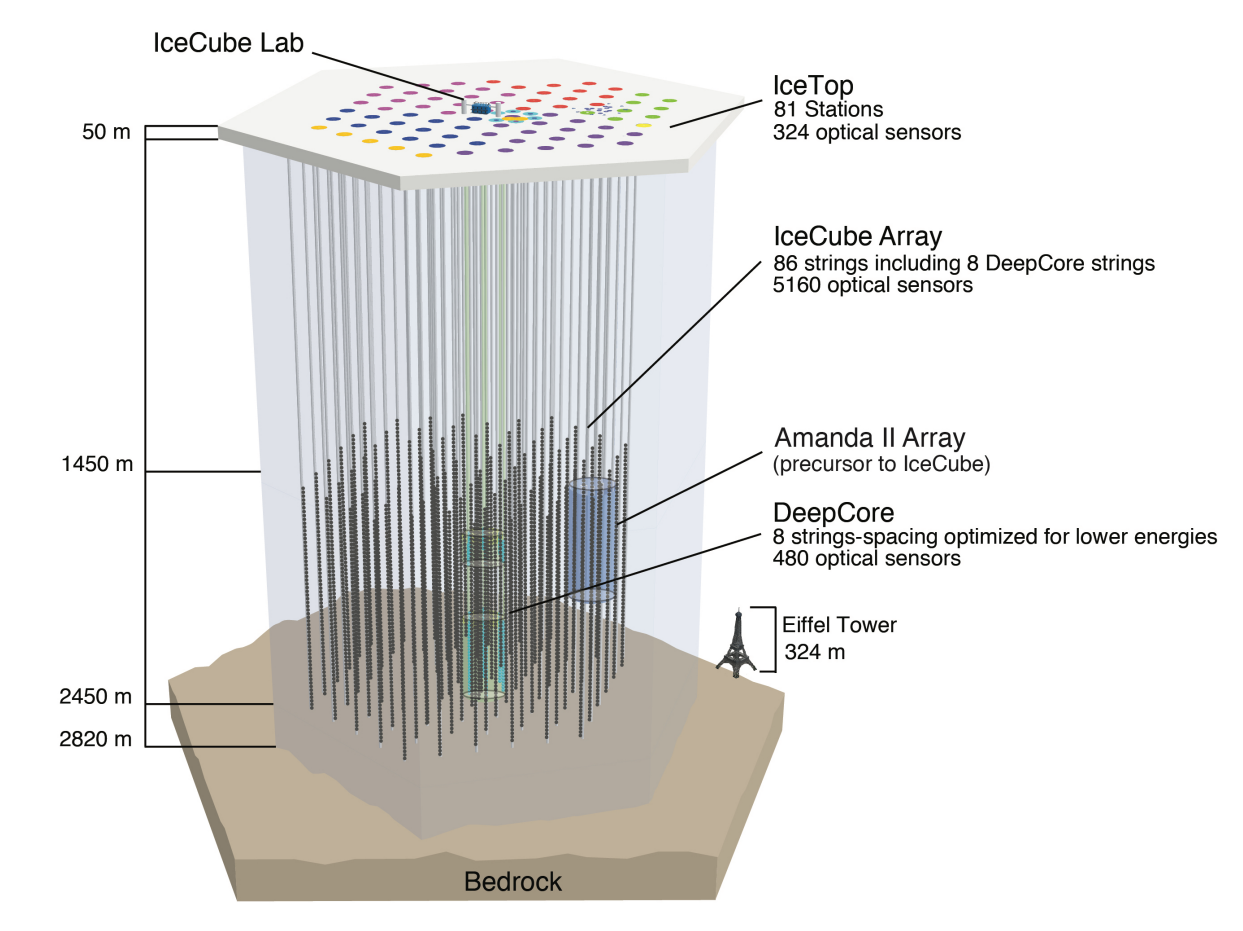
\includegraphics[width = 0.5\textwidth]{Ice_cube_layot.png}
    \caption{The ICE CUBE neutrino observatory. The detector is located at the south pole and is a large block of ice instrumented with photomultiplier tubes. Image taken from \cite{Andeen_2019}}
    \label{fig:Ice_cube}
\end{figure}

Neutrinos are weakly interacting matter particles and therefore are very difficult to detect. This makes them excellent candidates for the study of the Universe since they can travel large distances without interacting, but make them 
quite difficult to detect with high accuracy. The most famous detector and the one used in this paper is the ICE CUBE neutrino observatory. This detector is precisely what it sounds. It is a large block of ice located at the south pole.
The observatory uses the ice located deep in the South Pole as a giant Cherenkov detector. The ice is instrumented with photomultiplier tubes that can detect the Cherenkov radiation produced by neutrinos interacting with the ice. 
More precisely the observatory is fitted with 5160 photomultiplier tubes located at a depth of 1450-2450 m. The photomultipliers are divided into 86 strings of 60 modules each. The detector is also complemented by the DeepCore detector which is a denser array of photomultiplier tubes located in the center of the detector. See figure \ref{fig:Ice_cube} for a visual representation of the detector.
The energy range for this detector is from 10 GeV to 10 EeV. The interaction of neutrinos with the water molecules in the ice can produce charged leptons( muons, electrons or taus). These charged particles if energetic enough will then produce Cherenkov radiation which can be detected by the photomultiplier tubes.


\subsubsection{Emissivity estimates}
\label{sec:emmisivity_neutrinos}

Armed with the required knowledge above one can also make simple arguments for the sources of these neutrinos based on the observed 
flux here on Earth. The flux used in this paper is the diffuse flux of neutrinos as measured by the Ice Cube observatory. The flux is shown in figure \ref{fig:flux_neutrinos}. 
For any calculations, we use the astrophysical flux as modeled as a power law. The power law is on the form 

\begin{equation}
    \Phi(E) = \Phi_0 \left(\frac{E}{E_0}\right)^{-\gamma}
\end{equation}

with $\Phi_0$ being the normalization constant, $E_0$ being the reference energy and $\gamma$ being the spectral index. The model parameters are seen in table \ref{tab:neutrino_flux}.

\begin{table}
    \centering
    \begin{tabular}{|c|c|c|}
        \hline
        $\Phi_0$ & $E_0$ & $\gamma$ \\
        \hline
        $6.7\times 10^{-18} GeV^{-1} cm^{-2} s^{-1} sr^{-1}$ & $100 TeV$ & 2.37 \\
        \hline
    \end{tabular}
    \caption{The model parameters for the astrophysical flux of neutrinos as measured by the Ice Cube observatory.}
    \label{tab:neutrino_flux}
\end{table}

The emissivity of neutrinos is calculated in the same way as for UHECRs. The only difference is the loss time. neutrinos do not lose energy in the same way as UHECRs and therefore the loss distance will be the size of the Universe. 
The modeled emissivity is then approximately $1.19 10{45} \quad erg/Mpc^3/yr$

\begin{figure}
    \centering
    \begin{subfigure}[b]{0.35\textwidth}
        \centering
        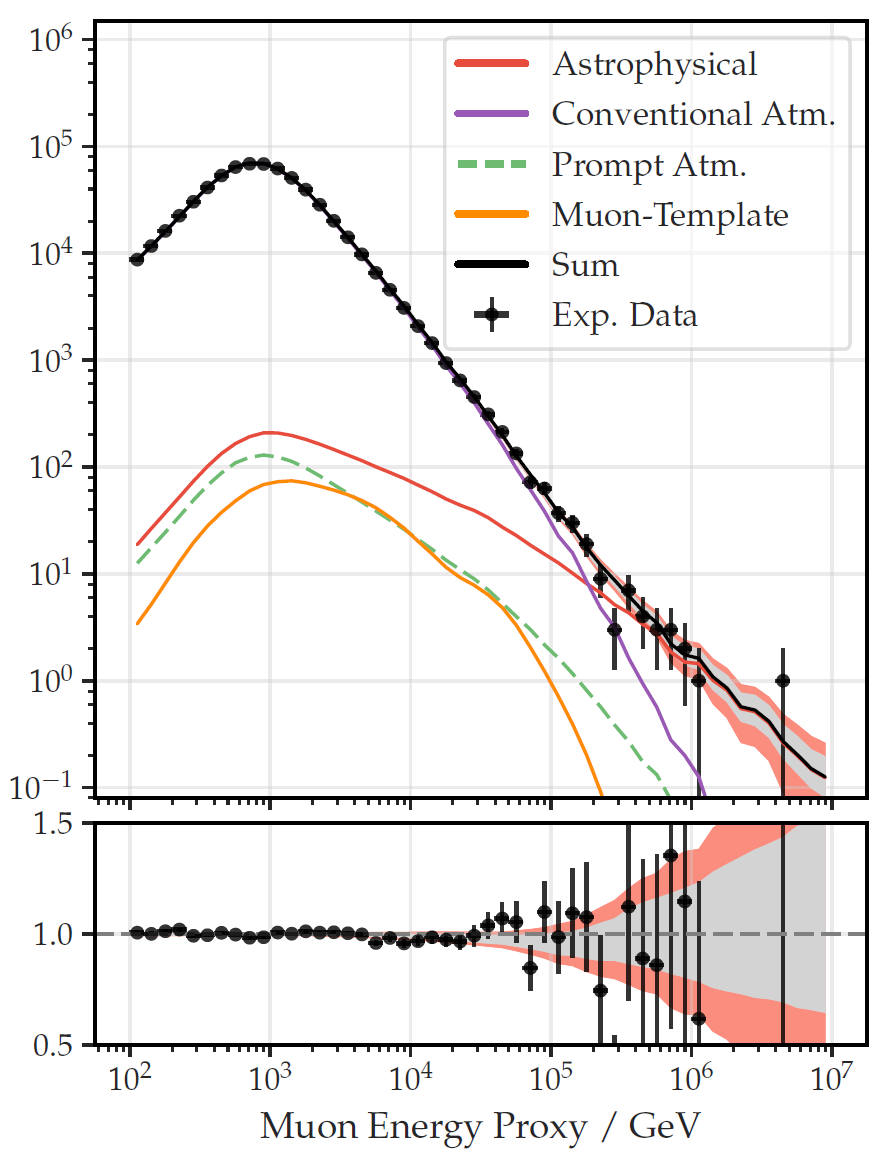
\includegraphics[width=\textwidth]{Ice_cube_flux_tot.png}
        \caption{Number of events per bin}
    \end{subfigure}%
    \begin{subfigure}[b]{0.5\textwidth}
        \centering
        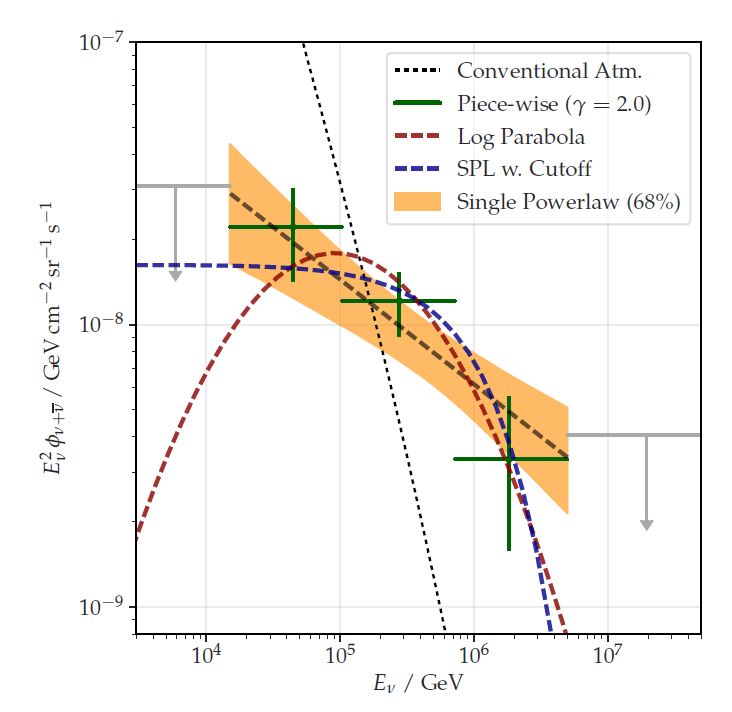
\includegraphics[width=\textwidth]{Ice_cube_flux_astro.png}
        \caption{Modeled Astrophysical flux}
    \end{subfigure}
    \caption{The diffuse flux of neutrinos as measured by the Ice Cube observatory. The y-axis on the left image is the number of events per bin.  The flux is separated into contributions from atmospheric neutrinos and astrophysical neutrinos. The right image is the model astrophysical flux as measured by ICE CUBE. Images taken from \cite{Abbasi_2022} }
    \label{fig:flux_neutrinos}
\end{figure}






\section{Active galactic nuclei}




Active Galactic Nuclei (AGNs) are an interesting field in astrophysical studies. 
Since their discovery, there has been rapid advancement in understanding these phenomena.
Today, AGNs are known to be among the brightest entities in the night sky,
but they only gained significant attention in the 1950s. 
This shift occurred with the arrival of new radio observations, which revealed a new type of quasi-stellar
object through the discovery of Quasars.

Initially, these luminous objects, characterized by broad, 
unidentifiable spectral lines, were enigmatic to scientists in the early 1960s. 
However, with the identification of more sources and their optical parts, 
it became clear that these were not stars but a distinct class of celestial objects. 
Research done by M. Schmidt on one of the emission lines from 
Quasar 3C 273 opened the interpretation of these celestial objects. 
He found that the emission lines of quasars were similar to hydrogen, but were redshifted by a factor of 0.158,
an exceptionally high value at the time \cite{Shields_1999}. Observations at the same time also revealed significant 
variability in quasar luminosity, suggesting that these objects were no larger than one light year across. 

These observations lead to the speculation of super luminous objects located very far away from Earth. The problem was that such objects
had no reasonable explanation at the time. It was not until the mid 1960 early 1970s when modern cosmology was 
afoot that more of these issues were resolved.

Observation of the surrounding galaxy of AGNs with matching redshift and observation of gravitational lensing cemented 
the distances of these objects. In addition, the modern view of black holes which had only been a theory in the 1950s came to
fruition and the modern model of an AGN was born. This modern perspective views AGNs as supermassive black holes that
accrete matter from surrounding accretion disks. This accretion releases large amounts of energy and has also according to 
processes such as the Blandford-Znajek process (1977), been shown to produce relativistic jets when the black hole is rotating.

In the most recent times, a landmark achievement was achieved in March 2021, when scientists associated with the Event Horizon Telescope project 
presented the first image of the supermassive black hole at the center of the Messier 87 galaxy, located 55 million light-years away.
This image, showing a bright ring surrounding a dark central region, aligns with predictions for an accreting supermassive black hole, 
reinforcing the understanding of these powerful cosmic sources.



\subsection{AGN structure and classification}


The modern view of AGNs is a unified model that combines different categories of powerful luminous objects visible in the night sky.
These distinctions that astronomers made still
have value, but to understand an AGN it is important to get a picture of the modern structure of an AGN

An active galactic nucleus is defined as a galaxy containing a massive accreting black hole. This mass according to \cite{Netzer_2015} 
is defined as $M_{BH} > 10^5 M_\odot$. AGNs also contain an Eddington ratio exceeding
the limit of $\frac{L_{AGN}}{L_{Edd}} = 10^{-5}$, where $L_{AGN}$ is the bolometric luminosity, and $L_{Edd}$ is the Eddington luminosity for a solar 
composition gas. These definitions help constrain what galaxies might contain an AGN, it excludes the Milky Way 
by these criteria, but it fails to capture the full structure definition of an AGN. 
Therefore the structure of most AGNs will include several of the following components. 

\begin{itemize}
    \item A close rotational dominated accretion disc around the SMBH. The thickness defining this accretion flow will distinguish different AGNs. 
    One example is an optical thin accretion disk that sometimes becomes advection-dominated.
    These flows will be referred to as radiation inefficient accretion flows(RIAF) due to the special nature of the disk.
    \item high-density gas clouds that are said to be dust-free moving at high velocities close to the black hole, in the so-called broad line region(BLR)
    \item Low-density gas clouds that move at lower velocities further away from the black hole in the so-called narrow line region(NLR)
    \item A axisymmetric structure of dust that is responsible for the obscuration of the central region of the AGN. This is called the torus.
     It lies at a luminosity-dependent distance from the SMBH, but according to \cite{Netzer_2015} this is around 0.1 - 10 pc depending on the luminosity.
    \item A corona of hot electrons that is thought to be responsible for the X-ray emission seen in AGN. This is thought to be located above the accretion disk. 
    \item A relativistic jet that is powered by the accretion disk. This is not always present but is a common feature of AGNs.


\end{itemize}
The reader is directed to image \ref{fig:my_label} for a visual representation of the different components.


\begin{figure}
    \centering
    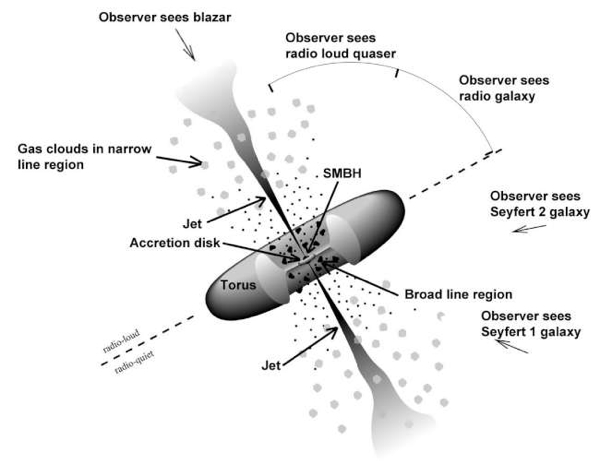
\includegraphics[width = 0.7\textwidth]{unified model agn.jpg}
    \caption{AGN unification}
    \label{fig:my_label}
\end{figure}

\subsubsection{Accretion disk}
An accretion disk is a natural consequence of the conservation of angular momentum. In the case of infalling 
matter coming close to a supermassive black hole, the matter will have some angular momentum. This angular momentum would in an ideal fluid orbit the black hole at some stable distance. Due to radative processes, fluid viscosity, and gravitational turbulence, 
the matter will lose angular momentum and spiral inwards. This inward spiral will eventually allow the matter to fall into the black hole. 
This process of inspiral is what is called accretion and the forces acting on the matter to cause the inspiral 
will also in the same process heat it up to high energies causing it to radiate. This radiation is closely linked to the 
infalling matter that is accreted onto the black hole and one can express the total luminosity of the accretion disk as 

\begin{equation}
    L_{acc} = \eta \dot{M}c^2
    \label{eq:accretion_luminosity}
\end{equation}

Here $\eta$ is the efficiency of the accretion disk, $\dot{M}$ is the mass accretion rate and $c$ is the speed of light.

The efficiency of the accretion disk is a function of the spin of the black hole and the radius of the innermost stable circular orbit (ISCO).
The ISCO is a counter-intuitive term in classical mechanics but in general relativity the maximum speed of a particle 
in addition to a energy term when calculating the orbit set bounds for how close a particle can be to 
a black hole without spiraling in. without going into to much detail the ISCO will be a solution of this equation based on the black holes mass and spin $a$

\begin{equation}
    6\frac{M}{r_{ISCO}}-8\frac{aM^(\frac{1}{2})}{r^{3/2}_{ISCO}}+3\frac{a^2}{r_{ISCO}^2} = 1
    \label{eq:ISCO}
\end{equation}
It is clear from \ref{eq:ISCO} that for a non-rotating black hole the ISCO takes the radius of $6M$, the result obtained from the calculation using the Swarzschild metric.


The accretion disk also has a bound for its maximum luminosity. As calculated for stars the Eddington
luminosity sets a maximum strength for the radiation pressure of the accretion disk. This is given as

Get sources!

\begin{equation}
    L_{Edd} = \frac{4\pi G M m_p c}{\sigma_T}
    \label{eq:eddington_luminosity}
\end{equation}

The heating of the accretion disc will lead to thermal radiation from the disc and this radiation will be
proportional to the temperature of the disc. This temperature is radially dependent and if one assumes an optically thick but geometrically thin disk also called a Shakura-Sunuaev disk
one can express the radiative surface energy flux taken from \cite{BHradiation}(p. 106) as 

\begin{equation}
    \frac{dE}{dAdt}= F_{rad}(r) = \frac{3GM\dot{M}}{8\pi r^3}\left(1-\beta\sqrt{\frac{r_{\rm ISCO}}{r}}\right)
\end{equation}

Here $\beta$ is a constant that relates the fraction of angular momentum captured by the black hole, and $r_{\rm ISCO}$ is the radius of the innermost stable circular orbit. 
The temperature of the disk lie between $10^5 - 10^2$ K with emission in the optical, UV to soft X-ray range. \cite{scholarpedia_accretion_discs}


\subsubsection{Corona and X-ray emission}
From highly varying x-ray observations of AGNs, it became indicative that there was a source of X-rays located close to the black hole. 
The most contemporary idea is that a corona of energetic particles is located above the accretion disk, and through inverse Compton scattering
of the optical/UV photons that arise from the accretion disk produce the seen x-ray emission. 

Inverse Compton scattering is the process of a photon gaining energy from a nearby relativistic particle. Due to the increase in efficiency 
of up scattering a photon with an electron compared to a proton, the corona is thought to be dominated by electrons. The process is as follows

\begin{equation}
    e^- + \gamma \rightarrow e^- + \gamma 
\end{equation}

The reason of interest for this area is that the correlation between the produced x-ray luminosity can be used to infer some luminosity of the more elusive 
particles UHECRs and neutrinos. The reason for this is that the ingredients for this x-ray production are the same as for the production of UHECRs and neutrinos (charged particles and photons). In addition, 
the acceleration into the jet-like structure of AGN needs a source of particles and the corona is a natural candidate for this.





%\subsubsection{Emmision lines}
%When a particle is photionized by the continuum radiation of a source it will emit a photon when it returns to its ground state. 
%This photon will have a specific wavelength that is determined by the energy difference between the two states.
%This wavelength is called the emmision line of the particle. When looking a dynamical systems with high velocities 
%the doppler shift of these emmision lines becomes important since it will affect the observed spectra of the source.

%https://lweb.cfa.harvard.edu/~pberlind/whipple/agn.html



\subsubsection{Broad and narrow lines region}

Broad emission lines in the case of AGN are formed from the high-density gas clouds located close the the central black hole. The 
high-density parameter is inferred from the fact that one only sees broad emission from permitted line transitions (f.ex hydrogen Lyman and Balmer,
iron II, and magnesium II). High densities allow for collisional de-excitation and in doing so prohibit so-called forbidden transitions.
The broadening is an indication that these gas clouds are moving at huge velocities around the massive objects. This implies that they are located close to the black hole and receive the name the broad line region

Narrow emission lines are on the other hand formed in low-density gas clouds. The low densities are inferred from the fact that one sees
both permitted and forbidden line transitions. They are narrow lines due to their velocities being substantially lower than the innermost gas clouds, and from here are thought to be located further away from the black hole, in the narrow line region. 


\subsubsection{dust torus}
%https://www.sciencedirect.com/science/article/pii/S0032063315000483#:~:text=This%20model%20proposes%20that%20all,collimating%20the%20radiation%20that%20escapes

The dust torus is a structure of dust that is thought to be located quite close to the black hole (0.1 - 10 pc). The main argument for the existence of this structure is the obscuration of the central region of the AGN. This obscuration 
is part of the unification scheme of AGNs and was backed by the detection of polarized broad lines in AGNs with their central core obscured. This polarization is what we would expect if some dust was obscuring the central region since the only light one sees is 
the light that is scattered into the line of sight \cite{MASON201597}. Further studies on the dust torus have also revealed that the torus is not uniform but clumpy and quite dynamic with both in and outflows of matter depending on the state of the central engine \cite{MASON201597}. 





\subsubsection{Jets}
\label{sec:jets}

A jet is a highly collimated outflow of plasma. The origin of the plasma is thought to be the accretion disk and the hot corona above it. These regions that have a high density of charged particles will under the influence of a magnetic field be accelerated and collimated into a jet-like structure.
The energy mechanism which powers the jet is not fully understood but the most prevalent theory is the Blandford-Znajek process. It says that the rotation of the accretion disk induces a magnetic field that will interact with a rotating black hole, effectively extracting energy from the black hole and supplying it to the jet. 
The jet structure extends far beyond the local area of the AGN maintaining a stable configuration over these distances. The classification of these jets is usually divided into two groups, FRI and FRII. They are differentiated by their luminosity where FRI jets are less luminous and have a more diffuse structure while FRII jets are more luminous and have a more stable structure reaching further out. \cite{walg2013relativistic}.
To add to this distinction it is thought that FRII jets are a product of an efficient accretion disk while FRI jets are a product of an inefficient accretion disk. This is discussed in \cite{Wei-Hao_2003} where they show that radio quiet and sefyert 1 galaxies have lower accretion efficiency while radio loud galaxies have higher accretion efficiency. 
Beyond the energy and their structure, the jets are also notable for their emission of non-thermal radiation such as synchrotron and inverse Compton radiation. They are also thought to be a possible source of UHECRs and neutrinos.







\subsection{Types of AGNs}

Before the unification of the AGNs astronomers named the puzzling objects based on their observational properties. These 
names are still used to this day and are somewhat useful since their observational properties are important parameters for further study. 
The different classifications are important in understanding which objects could have the potential to produce the different observables one 
looks for in the night sky. Therefore it seems appropriate to
discuss the different types of AGNs and their observational properties. The classification in this section is based on \cite{Astrobites}.

\textbf{Type I and II AGNs}:
One distinguishes type I and type II AGNs based on the presence of broad emission lines. In other words, this distinction is
a matter of a visible nucleus or not. Type I refers to sources whose nucleus is exposed to the observer and whose spectrum
has both narrow and broad emission lines. Type II refers to sources whose nucleus is obscured by a torus and therefore only has narrow emission lines.

\textbf{Blazars}:
The most extreme class of AGN. These sources are distinguished by their relativistic jets that are pointed towards the observer. 
This jet produces both synchrotron and Inverse Compton gamma rays and are extremely variable over short timescales. The
emission is also highly polarized. Often and including in this paper one divides blazars into subgroups based on the 
emission lines. The two most common are BL Lacs and Flat spectrum radio quasars (FSRQs). The difference between these two is the
presence of broad emission lines, where BL Lacs have no broad emission lines while FSRQs do. 
In addition the distinction comes from the type of jet structure thught to be associated with the source. FRI jets for Bl lacs and FRII for FSRQs. 

\textbf{Radio galaxies}:
As the name suggests these sources are very bright in the radio band. They usually refer to AGN viewed edge-on, where the
torus might block the emissions from the accretion disk. The orientation of Radio galaxies gives way to strong 
synchrotron radiation, and they are often used to study the jet structure of AGNs.

\textbf{Seyfert galaxies}:
Spiral galaxies that have a bright nucleus. They are bright in the optical band and have a smaller active region 
than radio galaxies. They are often divided into two groups Seyfert I and Seyfert II where the distinction comes from type I and II. 
They also show quite high variability indicating a small emmiting region. 

\textbf{Compton thin AGNs}: 
Not a common way of distinguishing AGNs but used in this rapport. These AGNs have lower absorption compared to Compton-thick AGNs, which allow more X-rays to escape. 

%https://iopscience.iop.org/article/10.1086/305813/fulltext/37493.text.html#:~:text=,line%20time%20delays%2C%20or%20lags


All these different distinctions are a help in understanding what processes one might be observing. The different
dominant bands indicate different processes being in the line of sight, and by considering the modern structure of 
AGNs one can then try to determine the underlying dynamics.  

 



\section{ Luminosity functions}
In this section, we will discuss the use of luminosity functions to characterize the populations of different AGNs. 
A luminosity function (LF) is a function that maps the distribution of celestial bodies, like galaxies or quasars,
based on their luminosity and corresponding comoving volume elements. These functions serve as a tool to understand the evolutionary patterns of these objects and allow us 
to predict the number density of these objects. 

%The function describes how a population varies based on luminosity but also crucially on its comoving volume element. 
Typically, the focus is on the differential luminosity function, which is defined as
\begin{equation}
    \frac{d\Psi(L,z)}{dL} = \frac{d^2N(L,V_c(z))}{dLdV_c(z)}
\end{equation}

%The quantity of interest is now a number density which can be very useful in deriving observed flux of different objects here on earth. 
One also can change the differential of the comoving volume into a term only depending on the redshift assuming the source population is isotropic and by multiplying with the differential comoving volume element. This 
transformation goes as follows, 

\begin{equation}
    \frac{d^2N(L,V_c(z))}{dLdV_c(z)}\frac{dV_c(z)}{dz} = \frac{N(L,z)}{dLdz}
\end{equation}


Several articles express the luminosity function in base $10$ logarithm and we note the conversion between the two:


\begin{equation}
    \frac{d\Psi(L,z)}{dLog(L)} =  \ln (10)  Lx \frac{d\Psi(L,z)}{d(L)}
\end{equation}


To effectively determine the LF, it's typically divided into two distinct components: a local term and a time evolution term.
 This approach involves taking the local luminosity function, calculated at a redshift 
$z=0$
, and then scaling it with a function that accounts for redshift evolution. 
The exact form of the total LF varies based on the source object, but it generally falls into two categories derived from the method of incorporating the evolution term into the local LF.
 These methods are selected based on which best represents the observed evolution.

 The two distinctions are the Pure Density Evolution (PDE) and the Pure Luminosity Evolution (PLE). 
 The PDE model modifies the local density function to reflect changes over time, 
 while the PLE model adjusts the local luminosity. The evolution is better represented by their equations and is given as 

\begin{equation}\frac{d\Psi(L,z)}{d(L)} = 
    \begin{cases}
        \frac{d\Psi(L/e(z),z=0)}{d(L)} \quad (PLE)\\
        \frac{d\Psi(L,z=0)}{d(L)}e(z) \quad (PDE)\\
    \end{cases}
\end{equation}

Here one sees the common way of representing the luminosity functions. The local luminosity function is scaled by a factor of $e(z)$ which is the evolution term.
\subsection{X-ray LF}

\begin{table}
\centering
\title{Parameter values for the X-ray luminosity functions}
\begin{tabularx}{\textwidth}{|l|XXXX|XXXXX|}
\hline

& \multicolumn{2}{c}{\textbf{LF params}} &&&  \textbf{Evolution params} &&&&\\

\textbf{Model} & $A$ & $L_{star}$ & $\gamma _1$ &  $\gamma _2$  & $v_1$ & $v_2$ & $z_c$ & $L_c$ & $ \alpha$\\
\hline
SLDDE RG & $8.375^a$ & $2.138^b$ & 2.15 & 1.10 & 4.00 & -1.50 & 1.90 & $3.981^b$ & 0.317  \\

AMPLE-Blazar & $1.379^a$ & $1.810^b$ & -0.87 & 2.73 & 3.45 & -0.25 & & &  \\

AMPLE-FSRQ & $0.175^a$ & $2.420^b$ & -50.00 & 2.49 & 3.67 & -0.30 & & &  \\

APLE-BLlac & $0.830^a$& $1.000^b$ & 2.61 & &-0.79& & & &  \\
APLE-Seyfert & $0.909^b$ & $0.61^b$ & 0.8 & 2.67& & & & &  \\
ULDDE-CTN AGN$^c$ & $2.91^a$ & $0.93^b$ & 0.96 & 2.71& 4.78 &-1.5 &1.86 &$4.07^b$ &0.29  \\
\hline
\end{tabularx}
\caption{X-ray LF parameters, $a)$ normalised by a factor of $10^{-7}$, $b)$ normalised by a factor of $10^{44}$
c) has more factors that do not fit in the table, $z_{c2} = 3$, $\alpha_2 =-0.1$, $L_{c2} = 10^{44}$, $v_3 = -6.2 $, $\beta=0.84$ }
\label{tab:xray_lf}
\end{table}

\begin{table}
    \centering
    \begin{tabular}{ll}
    \hline
     Model Name   & Luminosity Range (Log(L))  \\
    \hline
     SLDDE RG     & 42 - 47            \\
     AMPLE Blazar & 43 - 49          \\
     AMPLE FSRQ   & 45.5 - 49          \\
     APLE BLlac   & 44.5 - 49        \\
     APLE Seyfert & 41 - 47          \\
     ULDDE All AGN & 42 - 46 \\
    \hline

\end{tabular}
\caption{Luminosity range for different models}

\label{tab:lum_range}

\end{table}


%One way of calculating the neutrino flux of AGNs is based on their connecting with x-ray radiation. 
%Therefore in some literature, it is of interest to define the x-ray luminosity function for AGNs.

For a given type of celestial object, different spectral bands will be more useful than others. In the case of AGNs, 
the X-ray band is particularly significant. Therefore, several studies have focused on defining the luminosity functions of AGNs with the X-ray spectrum.

In the following, I will define the x-ray luminosity functions for various AGN classifications, including Radio Galaxies, Seyfert Galaxies, and Blazars. Furthermore, an additional breakdown will consider Flat Spectrum Radio Quasars (FSRQs) and BL Lacertae objects (BL Lacs) within Blazars.  In addition to this, 
a study by \cite{Ueda_2014} also looked at the total evolution of all Compton-thin AGNs by combining multiple surveys and research.  It will work as a reference point as well as describe the total evolution of these objects. The luminosity functions are collected from three papers \cite{Ajello_2009} and \cite{Silverman_2008}, and \cite{Ueda_2014} and their form is explained below.

\textbf{The local luminosity function}:

The local luminosity function is the luminosity function at $z=0$.
The simplest form of the local luminosity function is expressed in \cite{Ajello_2009} and is given as a power law. For our classes, it represents only the local LF for the class of BL Lacs 
and is given as

\begin{equation}
    \frac{d\Psi(L,z=0)}{dL} = \frac{A}{L_x} \left( \frac{L_x}{L_*}\right)^{1-\gamma_2}
\end{equation}

This functional form has the fewest parameters and therefore suits well for populations that have few detected sources, but has the disadvantage of not being able to capture all the details of the observed local luminosity functions when source counts increase.
For that reason a more complex local function is needed which was proposed in \cite{Ueda_2003} and is described by a double power law.
The double power law is used for the remaining classes of AGN and is given as follows


   
\begin{equation}
    \frac{d\Psi(L,z=0)}{dL} =  \frac{A}{\log(10)} \frac{1}{L_x} \left( \left( \frac{L_x}{L_*} \right)^{\gamma_1} + \left( \frac{L_x}{L_*} \right)^{\gamma_2} \right)^{-1}
\end{equation}

%The double power law introduced a break in the form of the local LF. This break is located at $L_*$ and is the luminosity where the slope of the LF changes. 


\textbf{Evolution factor}:

In addition to the local LF one also considers the evolution factor denoted $e(z)$. This factor captures the observed evolution of these objects and is the second part of the total luminosity function.

Again for the simplest evolution with the fewest parameters, a power law is used.
 $$
e(z) = (1 + z)^{v_1 }
 $$


  
Certain situations necessitate a more detailed approach to the redshift evolution. 
 As detailed in \cite{Ajello_2009}, a modified evolution is frequently employed. 
 This adaptation transforms the conventional Pure Luminosity Evolution (PLE) and Pure Density Evolution 
 (PDE) into their modified counterparts, namely Modified PLE (MPLE) and Modified PDE (MPDE).
It is within these modified frameworks that a dependence on redshift $z$ emerges in the exponent,
providing a more nuanced understanding of the evolutionary processes involved. It is given as

$$
e(z) = (1 + z)^{v_1 +v_2 z }
 $$



 To expand further as described in \cite{Silverman_2008} the evolution factor of the luminosity function is not always as simple as a modified power law only dependent on the redshift $z$.
For some sources, a more complex evolution is needed. In \cite{Silverman_2008} they use a double power law to better fit the data where 
 the evolution is now not only dependent on the redshift but also on the luminosity. This then receives the apt name as a luminosity-dependent density evolution (LDDE) since it is a modified version of a (PDE)
 The functional form of the LDDE is as follows


 \begin{equation}
    e_z(z, L) = 
    \begin{cases} 
    (1 + z)^{v_1} & \text{if } z \leq z_*(L) \\
    e_z(z_*(L), L) \times \left( \frac{1 + z}{1 + z_*(L)} \right)^{v_2} & \text{if } z >  z_*(L)
    \end{cases}
 \end{equation}

 with $z(L)$ being defined as

 \begin{equation}
    z_*(L) = 
    \begin{cases} 
    z_c \left( \frac{L}{L_c} \right)^\alpha & \text{if } L \leq L_c \\
    z_c & \text{if } L > L_c 
    \end{cases}
 \end{equation}


 The expansion of the parameter space allows for easier fitting to the observed data, but comes of course with an increase in complexity and possible over fitting. 

 Lastly \cite{Ueda_2014} considered an XLF for the entire population of AGNs and naturally this has a more complex evolution structure. It is also an LDDE model but with three steps instead of two which we have in \cite{Silverman_2008}.
The evolution is given as

 
\begin{equation}
e_z(z, L) = 
\begin{cases} 
(1 + z)^{p_1} & \text{if } z \leq z_*(L) \\
(1 + z_{*})^{p_1} \left( \frac{1 + z}{1 + z_*(L)} \right)^{v_2} & \text{if } z >  z_*(L)\\
(1 + z_{*})^{p_1} (\frac{1 + z_{*2}}{1+ z_{*}})^{v_2} (\frac{1+z}{1+z_{*2}})^{v_3} & \text{if } z >  z_{*2}(L)

\end{cases}
\end{equation}

with the exponent $p_1$ being defined as
\begin{equation}
    p_1 = v_1 + \beta(log(L)-44)
\end{equation}

with $z_{*}(L)$ being defined as

\begin{equation}
z_*(L) = 
\begin{cases} 
z_c \left( \frac{L}{L_c} \right)^\alpha & \text{if } L \leq L_c \\
z_c & \text{if } L > L_c 
\end{cases}
\end{equation}


and $z_{*2}(L)$ being defined as

\begin{equation}
z_{*2}(L) =
\begin{cases}
z_{c2} \left( \frac{L}{L_{c2}} \right)^{\alpha_2} & \text{if } L \leq L_{c2} \\
z_{c2} & \text{if } L > L_{c2}
\end{cases}
\end{equation}



Armed with the functional form of the total luminosity function one can now fit the parameters to the observed data. This is done in \cite{Silverman_2008}, \cite{Ajello_2009} and \cite{Ueda_2014} and their 
model name is a combination of the source paper (S, A, U), the type of model it describes (PLE, MPLE, LDDE) and the object in question. The parameters are then fitted to the data using a maximum likelihood method and the observational data of several x-ray surveys, see the cited papers for more information.
One can see the parameters for the different models in table \ref{tab:xray_lf} and the luminosity range for which the different models are valid in table \ref{tab:lum_range}. 




\section{Evolution}
In this section, we will be using the different luminosity functions from the previous section to calculate the evolution of the different classes of AGNs. 
This evolution illustrates the different distribution one can expect from the different classes across luminosity and redshift, highlighting their evolution in time and energy.
%By looking at the different trends for the different type of distributions one can observe the evolution and energy distribution of the different classes of AGNs. 


 


\subsection{Luminosity distribution}
 
For the different classes discussed one can integrate the differential luminosity function over redshift to retrieve the Luminosity distribution of each 
object. This distribution highlights the difference in emitting power and therefore is important for us to be able to distinguish the most powerful 
sources and their prevalence, and also any trends that might be interesting. One calculates the Luminosity density by multiplying the class-specific luminosity
function with the differential comoving volume and integrating over the relevant redshift bin. 
%that the evolution beyond the given luminosity range is not known and therefore the distribution is not complete. And deducing continued evolution
%can be done but must be taken with a grain of salt. The number of objects these functions are built upon are not very numberous and therefore
%the error bars are quite large, especially in the edges. 

The luminosity distribution is given as


\begin{equation}
    \frac{dN(L)}{dL} = \int_{z_{\text{min}}}^{z_{\text{max}}} \frac{\Psi(L, V(z))}{dL} \frac{dV(z)}{dz} dz
\end{equation}

Here, $z_min$ and $z_max$ are the limits of the redshift bin. By separating it into
bins of redshift one can asses how the dominant luminosity class varies with redshift, and how a change in redshift would change the slope/trend of the distribution.  
%It is important to note 


In figure \ref{fig:LD} one can see the luminosity density for the six different luminosity functions. The distribution is 
separated into four bins of redshift ($0<z<2,2<z<4,4<z<6,6<z<8$). %
%This is done to illuminate the evolution of the different classes at different epochs
The most interesting feature of these distributions is the difference between the break luminosity between jett-dominated classes such as blazars and emission-line classes such as radio galaxies and Seyferts.
For the jett-dominated ones the luminosity distribution breaks at a certain point and decreases on both sides. The only exception to this is the BL Lacs which are represented as a simple power law and therefore have no
break point in their distribution. With the discovery of more BL Lacs in the future it would be interesting to see if this is still the case. %The reason for the use of a single powerlaw for the BL Lacs is namly due to the lack of observations.  
The breakpoint for blazars and FSRQa indicates an energy value where these classes are the most numerous.
%An interesting point brought up in \cite{Ajello_2009} is the effect of beaming of X-rays for blazars. This effect flattens the XLF for lower luminositie. 



For the emission-line classes, one sees an increase towards lower energies, but they all have a break luminosity. The fact that these AGN classes all have a break luminosity is very interesting since it seems to show 
a breaking point where the birth of these sources becomes significantly harder and therefore less numerous. The increase in x-ray luminosity is tightly connected to the amount of accretion onto the black hole and therefore
a breakpoint in the energy production of similar sources is very interesting.
This breakpoint is for example seen in all CTN AGNs and radio galaxies and is also varying based on the redshift bin. For higher redshift, the break is more sudden. For the Seyferts that have no evolution factor there is no distinction between lower or higher redshift

The redshift bins for the blazar population show a very interesting trend. The amount of blazars at lower redshift seems to not change but passed the break point the total number of blazars becomes redshift dependent, where there is a big difference between the middle epochs and the others. 
This is also seen for the FSRQs, but the break luminosity is met with a much steeper decline. For Bl lacs, the redshift bins show a different trend. Here the number of sources is only increasing with redshift. 

For the study of these objects, the biggest takeaway in my opinion is the break luminosity and how one would reproduce it in a model. 



\subsection{Density distribution}

In addition to the luminosity distribution one can also calculate the number density of the different classes of AGNs. This is done by integrating the
differential luminosity function over luminosity. This will illuminate the evolution of the different classes of AGNs in terms of redshift. The integral is given as

\begin{equation}
    n(z) =\frac{N(z)}{V(z)} =  \int_{L_{\text{min}}}^{L_{\text{max}}} \frac{\Psi(L, V(z))}{dL} dL
\end{equation}

Here again, we separate into luminosity bins to see the evolution of different luminosity bins, most notably to see the difference before and after the break luminosity for most classes. 
The results can be seen in figure \ref*{fig:DD}






%\begin{figure}
%    \centering
%    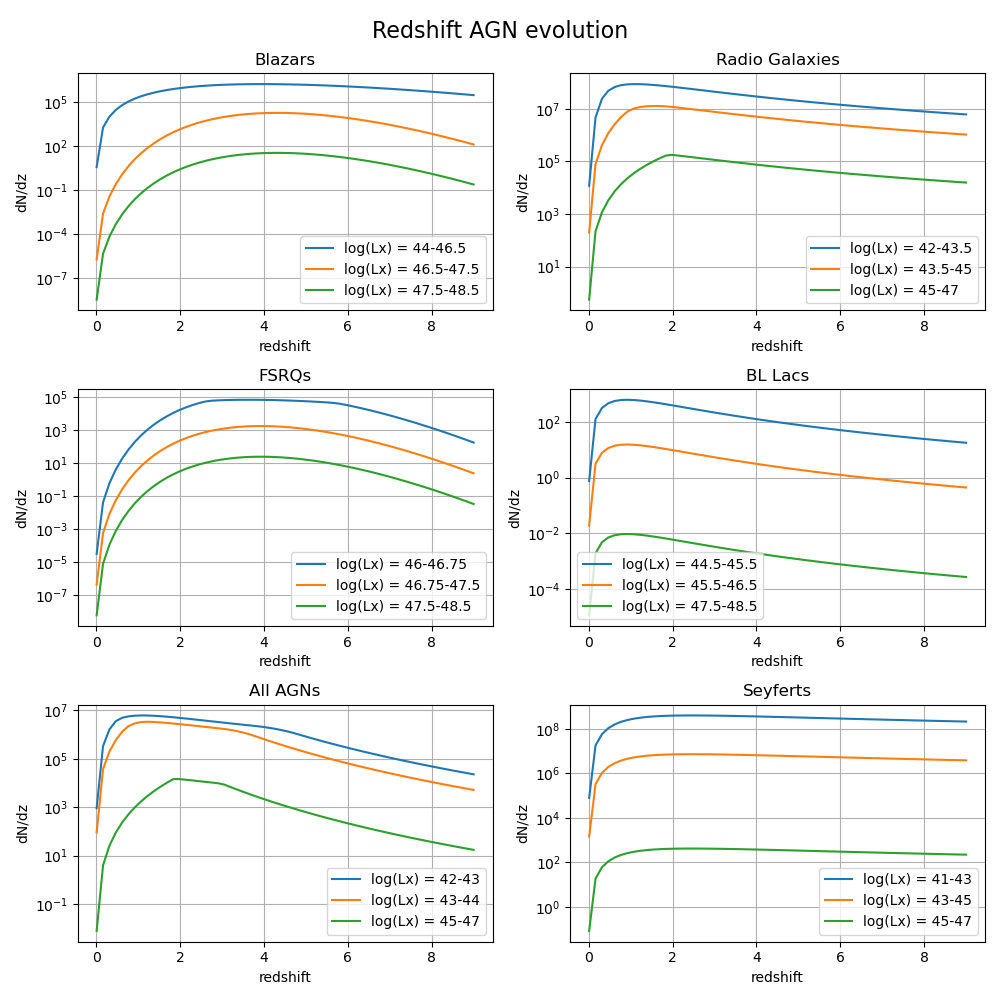
\includegraphics[width = \textwidth]{new_plots/Redshift AGN evolution.png}
%    \caption{Number evolution in terms of redshift for the four different classes of AGNs. The different classes are defined in the title as well as the chosen LF model.}
%    \label{fig:ND}
%\end{figure}



\begin{figure}[H]
    \centering
    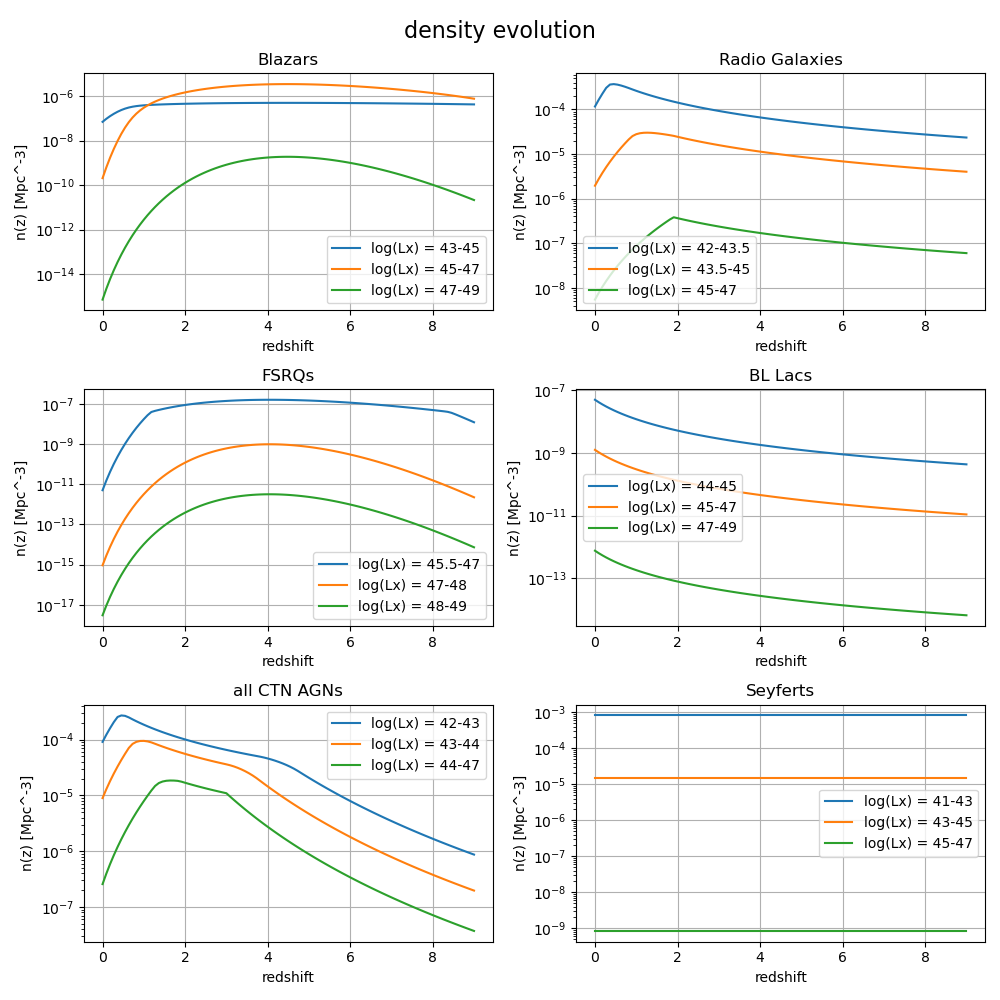
\includegraphics[width = \textwidth]{new_plots/Redshift density evolution.png}
    \caption{Density distribution for the four different classes of AGNs. The different classes are defined in the title as well as the chosen LF model.}
    \label{fig:DD}
\end{figure}



The density of these objects is arguably the most interesting part of this analysis due to it being closely tied to galaxy evolution. The evolution of blazars and FSRQs differentiate themselves significantly from the other classes in figure \ref*{fig:DD}
Both FSRQs and Blazars have a positive evolution with a peak in density around redshift $z=5$. The total counterpart to this is the third class of jet-dominated AGN, the Bl Lacs. Here one sees a negative evolution with 
and increase in density in the more recent epochs. According to \cite{Garofalo_2019} the origin of this discrepancy is the different evolutionary paths that generate the respective classes of Bl lacs and FSRQs. 
While both classes belong to the parent class of blazars the evolutionary path of FSRQs is thought to come from FRII radio galaxies while the evolutionary path of BL Lacs is from FRI radio galaxies. As mentioned in section \ref*{sec:jets} the correlation between FRI and FRII jets is thought to be the accretion efficiency. 
In addition to this \cite{Wei-Hao_2003} mentioned that this correlation might indicate the nature of the central black hole and its rotation. Drawing from this one could indicate that the difference in evolution stems from the different evolutionary paths of Kerr black holes (FRII) or Swarzschild black holes (FRI), plus the evolution of material that can be accreted around the central black hole.



For the blazar population, one notices the same trend as for the luminosity distribution. The luminosity bin before the break luminosity stays more constant than the ones after the break. The reason for such an evolution 
would likely be tied to the same mechanism driving Bl lacs and FSRQs. Due to the decline of FSRQs, one should also expect the
higher-end luminosity of blazars to follow.

For the emission-line AGNs, one finds a different story. Here the redshift peak, if any, is at around $z=0.3$ where the peak is dependent on the luminosity bin. Lower luminosity AGN peaks at lower redshift. Therefore the trend of density 
seems to be going toward lower-power radio galaxies and Compton-thin AGNs. 

What is also very interesting is comparing the evolution of all sources to 
the evolution of star formation. From \cite{Madau_2014} the star formation rate peaks at around 3.5 billion years after the Big Bang, 
or around redshift $z= 1.9$. This is in stark contrast to our sources where only the most luminous radio galaxies and Compton thin AGNs peak at this redshift. 
This is very interesting since then the presence of efficient accreting Kerr black holes such as our FSRQs would have been more numerous before the peak of star formation. 
And on the opposite side our CTN AGNs peak later. 


\subsubsection{Expected luminosity}
From the luminosity function, one can also calculate the expected luminosity of a source class at different redshifts. This is important since it will directly relate to the 
power injection of the different epochs and from this one can calculate an expected emissivity of the different classes of AGNs. 
The expected luminosity of each group can be calculated with the following formula

\begin{equation}
    \langle L \rangle = \frac{\int_{L_{\text{min}}}^{L_{\text{max}}} L \frac{\Psi(L, V(z))}{dL} \frac{dV(z)}{dz} dL}{\int_{L_{\text{min}}}^{L_{\text{max}}} \frac{\Psi(L, V(z))}{dL} \frac{dV(z)}{dz} dL}
\end{equation}

furthermore the emissivity is given as


\begin{equation}
     \epsilon  = \int_{L_{\text{min}}}^{L_{\text{max}}} L \frac{\Psi(L, V(z))}{dL} \frac{dV(z)}{dz} dL
\end{equation}

The different luminosity ranges are the same as before and are given in table \ref{tab:lum_range}. The results are shown in figure \ref{fig:EL}.

\begin{figure}
    \centering
    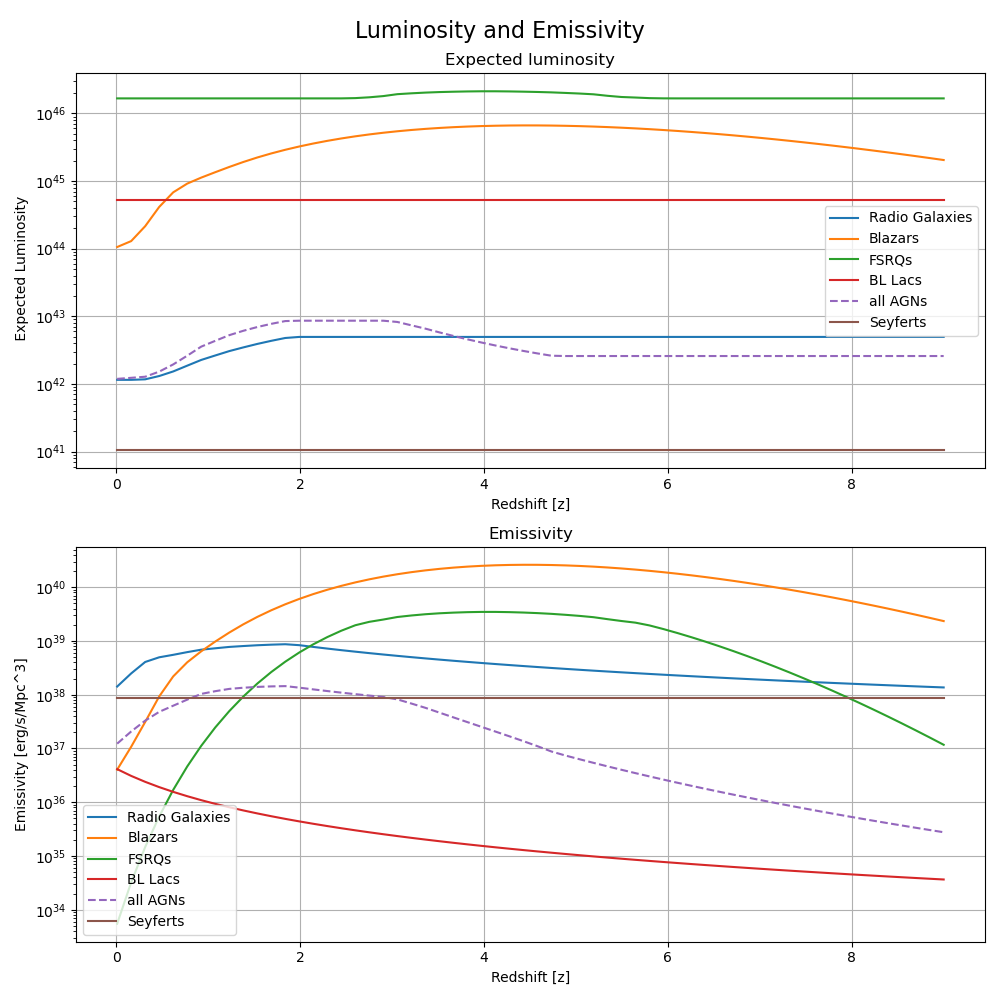
\includegraphics[width = 0.8\textwidth]{new_plots/Luminosity and Emissivity.png}
    \caption{Expected luminosity and emissivity for the four different classes of AGNs. The different classes are defined in the title as well as the chosen LF model.}
    \label{fig:EL}
\end{figure}



The expected luminosity is shown at the top in figure \ref*{fig:EL} where it shows the expected power output of the different classes. Here one sees that FSRQs are indeed the most luminous AGN and 
that they represent some of the most luminous objects in the Universe.
The expected luminosity also shows the evolutionary trend of blazars where they are now tending towards lower average luminosity. 
All classes remain fairly constant, but radio galaxies and CTN AGNs both have a decline in expected luminosity after the star formation peak at $z=1.9$. This could be inferred from figure \ref*{fig:DD} but is more clearly seen here.
The constancy of most objects across redshifts is comforting since it means that one could use a general model for any of the objects at any redshift without needing to account for the redshift. 
This is not the case for the blazars but since they are a combination of different objects any general model would be hard to find. On the other hand, any model for FSRQs and Bl lacs would not need to account for redshift and the varying parameters that come with that. 
%An important point to remeber is that this luminoisty is directly tied to the x-ray production of these sources. Therefore the expected luminoisty also shows us that 
%jett-dominated AGN produce more x-rays than emission-line AGN. This is not suprising but it is a indcication that these x-rays are not only produced in the hot corona, but also in the jet. 
%While for all compton thin AGNs one would expect the x-ray luminosity to be dominated by the hot corona.

The emissivity of each class as a function of redshift is shown in figure \ref*{fig:EL} at the bottom. This is effectively a combination of the number density of our sources and their respective expected luminosity. 
The figure shows a change in dominance between blazars and our CTN and radio galaxies. This change in dominance happens around redshift $z=1$ and is a result of the different evolution of the different classes.
This change is a direct result of the different evolutionary paths for our sources seen in figure \ref*{fig:DD} and should affect the diffuse astrophysical flux of UHECRs and neutrinos. 
The emissivity is a good indicator of what objects might dominate the different epochs and it is clear that at higher redshift $z>2$ our jet-dominated AGNs are the most powerful emitters of x-rays. 
An interesting point is how this increase in emissivity of different classes of AGNs would affect the outflow mechanism of the AGNs and how this would affect the surrounding galaxy. In \cite{Laha_2021}
they talk about the open questions regarding the outflow mechanism of AGNs and their feedback mechanism with their host galaxy. To add to these open questions one could ask how the change in x-ray emissivity in the different classes of AGNs would affect the same mechanisms.



\section{Excotic particle creation}
\subsection{UHECRS emmisivity}
With the calculated emissivity for the different groups, there is now the possibility to look from an energy budget viewpoint into the possibility of AGNs being the origin of UHECRs. The 
reasoning is quite simple but for the AGNs to be the origin of UHECRs they must be able to produce the necessary emissivity. 

From the calculation in \ref{sec:emmisivity} the emissivity of UHECRs is given as $1.73 \cdot 10^{44}\frac{\rm erg}{\rm Mpc^3yr \rm s }$ this was calculated from the observed flux of UHECRs from the Pierre Auger observatory \cite{thepierreaugercollaboration2017pierre}.
In this calculation, one needed to confine the area in which these sources could be produced to take into account the energy losses these particles experience. The same argument must be used 
for our emitting sources and therefore one must use the emissivity of our sources at a redshift very close to Earth. To get a comparable emissivity one evaluates therefore the emissivity at redshift $z=0.01$. The result is shown in figure \ref*{fig:flux_UHECRs}

\begin{figure}[H]
    \centering
    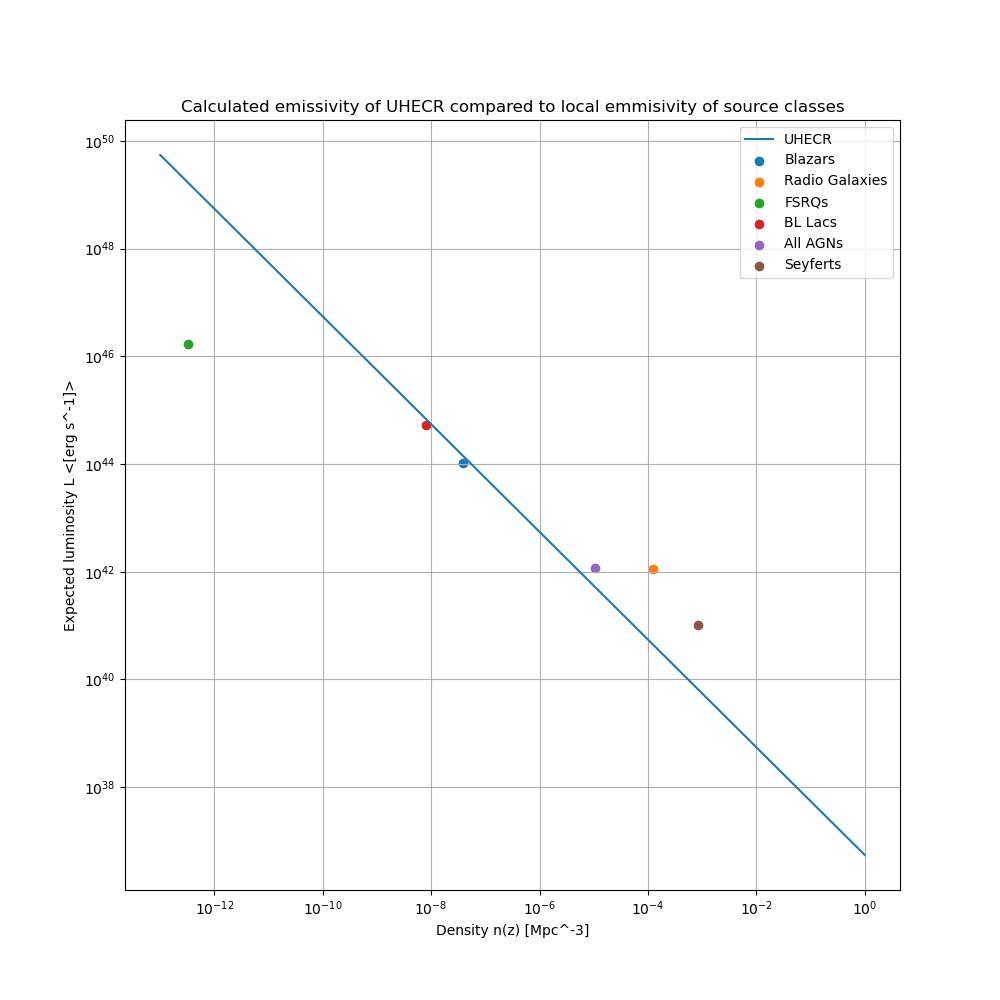
\includegraphics[width = 0.7\textwidth]{new_plots/L_n_uhecr_calc.png}
    \caption{UHECR emissivity for the four different classes of AGNs.}
    \label{fig:UHECR}
\end{figure}

This figure shows that most classes of AGN produce a total emissivity in X-ray comparable to the one energy detected by the Pierre Auger observatory. The only exception is the FSRQs which are not numerous enough at this redshift. 
To criticize this very crude estimate, one must first note that the correlation between X-ray luminosity and UHECR luminosity is not well defined and should include parameters that are not accounted for.
In addition to this one has not done any separation between jet-dominated and emission-line AGNs, and even though our emission-line AGNs are capable of producing the required x-ray luminosity
the mechanism of transferring this energy into UHECRs is not well understood. A very interesting point is that the only candidate not able to produce the required emissivity, the FSRQs, are the ones where according to \cite{Wei-Hao_2003} one could find a Kerr black hole. 
A Kerr black hole is needed in mechanisms such as the Blandford-Znajek mechanics which is a possible way of accelerating and beaming particles into jets. One notes that it is not only that mechanism that could accelerate UHECRs and 
the outflows discussed in \cite{Laha_2021} would have an acceleration mechanism as well. The author of this paper notes that the energy gain in these outflows is not known and therefore one cannot say if they are powerful enough to produce extra galactic UHECRs. 

Nevertheless, the result does not rule out the possibility of AGNs being the origin of UHECRs. 


\subsection{Neutrino emmisivity}
In a similar fashion for the UHECRs, we calculated the local emissivity for the neutrinos in section \ref{sec:emmisivity}. The result was $1.2 \cdot 10^{44}\frac{erg}{Mpc^3yr}$ which is a factor similar to that of UHECRs.
In the calculation, the diffuse neutrino flux on Earth was taken from the IceCube observatory \cite{Abbasi_2022} and the energy range was taken to be $1TeV - 10PeV$ corresponding to the astrophysical neutrino flux.
the difference between the UHECR flux to the neutrino flux is the energy loss mechanism. The effect of a very limited energy loss mechanism means that the emitting area is now the whole universe. To reach a comparable emissivity one must therefore take a redshift-dependent average of the sources over the whole universe.
One does this by scaling the emissivity at redshift $z$ with the corresponding energy loss for a neutrino from that redshift given as $(1+z)$ and then taking the average emissivity to get a comparable emissivity.
The resulting figure is shown in figure \ref{fig:neutrino}.

\begin{figure}[H]
    \centering
    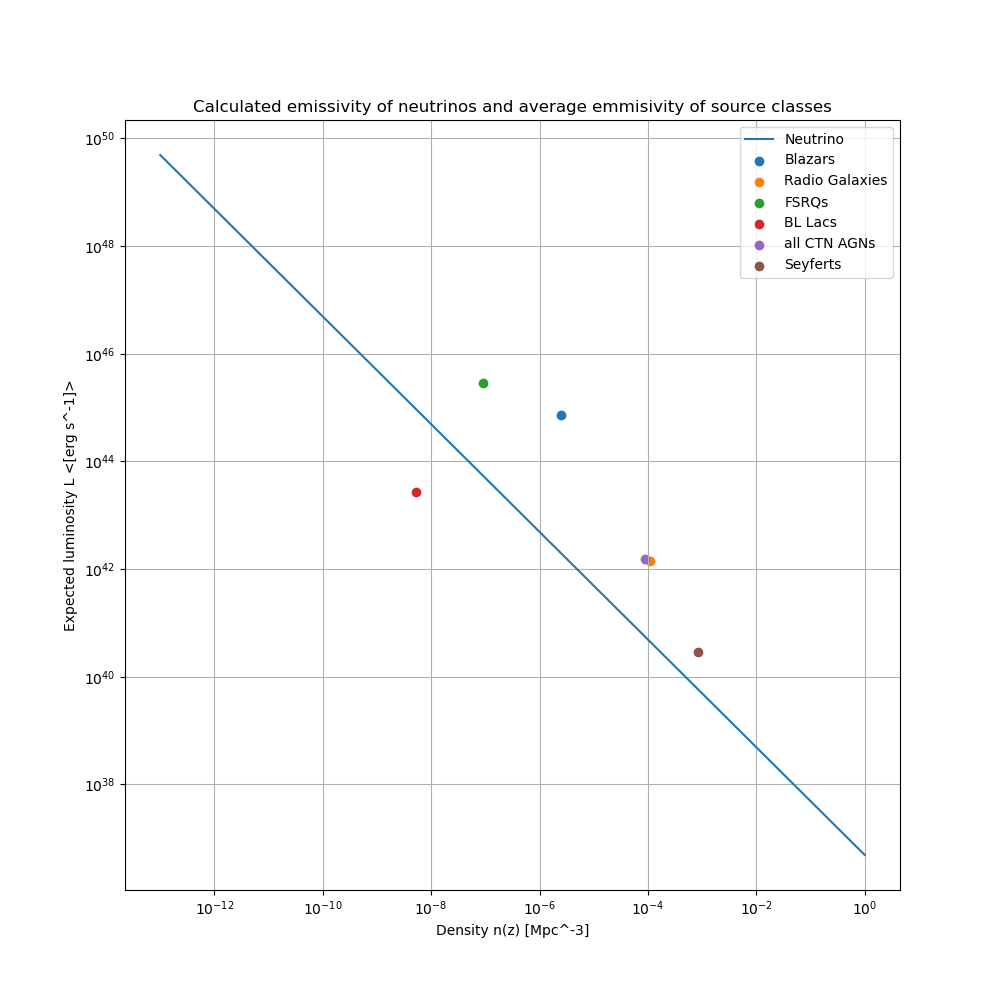
\includegraphics[width = 0.7\textwidth]{new_plots/L_n_neut_calc.png}
    \caption{Neutrino emissivity for the four different classes of AGNs.}
    \label{fig:neutrino}
\end{figure}

This figure shows that the neutrino flux can be produced by all classes except 
the BL Lacs. This is an effect of the averaging since the BL lacs have a negative evolution.
The opposite is the FSRQs which now can produce the required emissivity.

In addition to the average picture given in figure \ref*{fig:neutrino} one can also calculate the diffuse neutrino flux from the different classes of AGNs. This is done by modifying the transfer function defined in \cite{Palladino_2020} and this is given as


\begin{equation}
    \frac{d\phi_\nu}{dE_\nu} = \int_0^{z_{max}} \frac{D_H}{E(z)} \frac{L(E_\nu (1+z),<L_x>(z))}{(1+z)^2} \rho(z) dz
\end{equation}

Here $D_H$ is the Hubble distance, $E(z)$ is the function defined in section \ref{sec:comoving_distance}, $L(E_\nu (1+z), <L_x>(z))$ is a power law representing the neutrino flux at the source, which when integrated reproduces the average source luminosity at redshift $z$, and $\rho(z)$ is the number density of the sources at redshift $z$.
with this function, we can calculate the expected diffuse flux of neutrinos from the sources. The difference between \cite{Palladino_2020} and I, is the inclusion of a luminosity dependence in the power-law function. This is done to account for the different average luminosity of the different classes of AGNs which was assumed constant in \cite{Palladino_2020}. 
The assumption of a constant luminosity is not a bad one since the luminosity of the different classes is not changing significantly over the redshift range, but it is still a simplification, especially for the blazar class. The form of the spectra is taken to be identical to the observed neutrino flux by ICE CUBE which is defined in section \ref*{sec:emmisivity_neutrinos}.
The result is shown in figure \ref{fig:neutrino_diffuse}.
\begin{figure}[H]
    \centering
    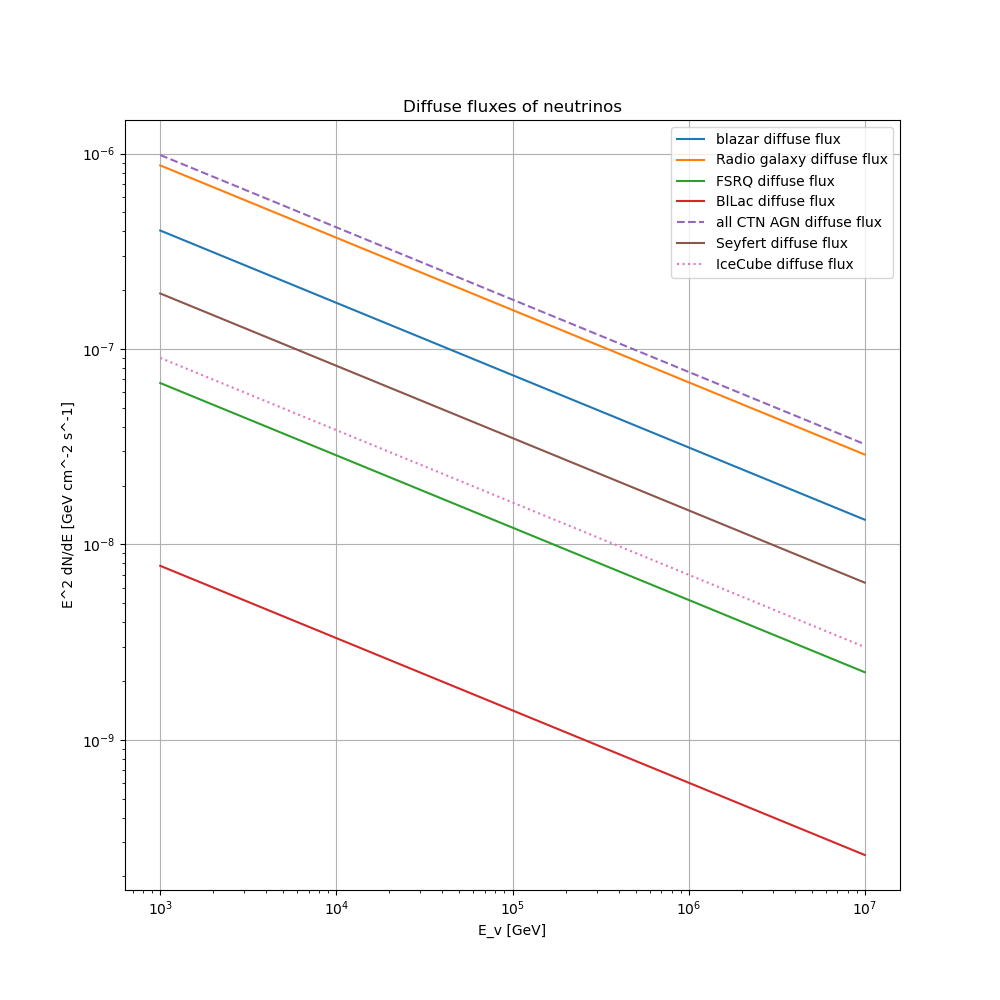
\includegraphics[width = 0.7\textwidth]{new_plots/diffuse_fluxes_neutrino_no_cutoff.png}
    \caption{Diffuse neutrino flux for the four different classes of AGNs.}
    \label{fig:neutrino_diffuse}
\end{figure}

what one sees here is almost the same result as the crude average which is good. The FSRQs and Bl lacs are now not able to produce the diffuse flux but the rest are. 
The fact that all sources are overshooting the observed neutrino flux would be a problem if we had a more constrained solution. Any model that overshoots could not be the source since it is not what we observe, but in our case, 
our solution rests on the fact that the neutrino luminosity is equal to the x-ray, an assumption easily broken and without nuance. Therefore the only concrete conclusion one can draw from this is that the neutrino flux can be produced by the AGNs since they can produce the required emissivity.
Several papers such as \cite{Kurahashi_2022} talk about the lack of any anisotropy in the observed diffuse neutrino flux. Such an anisotropy would introduce a required density of sources. This would be a problem for the more obscure sources such as FSRQs and could further limit our predictions.

This result in figure \ref*{fig:flux_neutrinos} is obtained differently than in figure \ref*{fig:neutrino} and therefore the agreement between them is a good sign. The argument that the x-ray luminosity should have the same value as the neutrino luminosity is not a bad first guess, but it does leave a lot to be desired. 
This flux model does not incorporate any parameters of the AGN other than emitting strength and therefore it is not a very nuanced model. A first fix could be a model that includes the jet orientation and most importantly the acceleration mechanism one could imagine happening. What this 
crude model can show is that these objects do produce enough power. To make the estimation better without doing much more work, one could look at the gamma-ray luminosity functions of the same sources and see if they can produce the required neutrino flux. Gamma-ray production is a natural consequence if one is using the pion decay model with the proton delta resonance
for neutrino production. In this way, one could more easily constrain the neutrino production with the gamma-ray production. 
This is however outside the scope of this paper and will be left for future work. 

\subsubsection{AGN as the origin of the astrophysical particles}
Both the diffuse flux of neutrinos and UHECRs estimate an emissivity that is comparable to the x-ray emissivity of our sources. The correlation between x-ray luminosity and the production of these ultra-high energy 
particles is also not unfounded since both require a high number of charged particles. For these arguments, one could imagine that AGNs of all classes can produce these particles. 

\section{Conclusion}

\bibliography{bib}
\bibliographystyle{apalike}

\end{document}
